% %
% RTXIMANUAL.TEX - reference manual for Real-Time eXperiment Interface v1.3
%                                       2011-04-04
%
%  Updated for REFMAN.CLS
%
\documentclass[twoside,letter]{refrep}
\usepackage{makeidx}
\usepackage{ifthen}
\usepackage[sort]{cite}
\usepackage{graphicx,epsfig}
\usepackage{textcomp}
\graphicspath{{./images/}} 
\usepackage[pdftex,bookmarks=true]{hyperref}

\def\tm{\leavevmode\hbox{$\rm {}^{TM} \;$}} % trademark
\def\bs{\char'134 } % backslash in \tt font.
\def\cpp{C\texttt{++}$\;$}

\newcommand{\ie}{i.\,e.,}
\newcommand{\eg}{e.\,g..}
\DeclareRobustCommand\cs[1]{\texttt{\char`\\#1}}

\title{Real-time eXperiment Interface (RTXI) \\User Guide\\
{\large RTXI v1.3}}

\author{Risa Lin}

\date{2011-08-31}
\emergencystretch1em  %

\pagestyle{myfootings}
\markboth{Real-time eXperiment Interface (RTXI)}%
         {Real-time eXperiment Interface (RTXI)}

\makeindex 

\setcounter{tocdepth}{2}

\begin{document}

\maketitle

%\begin{abstract}
%        This document describes the capabilities of the 
%        \texttt{refart} and \texttt{refrep} classes for \LaTeXe. 
%        These classes do not work with \LaTeX\ 2.09. They contain some 
%        improvements over the original \texttt{refman} style which may result 
%        in different output and minor incompatibilities, but make refman 
%        work with paper sizes other than ISO A4, which I consider an 
%        improvement.
%\end{abstract}

This file documents the Real-time eXperiment Interface (RTXI), a program for hard real-time data acquisition and control applications in biological research.

Copyright \copyright 2011\\
Boston University\\
Georgia Institute of Technology\\
Weill Cornell Medical College


This edition of the RTXI documentation is consistent with RTXI v1.3.

Permission is granted to make and distribute verbatim copies of this manual provided the copyright notice and this permission notice are preserved on all copies.

Permission is granted to copy and distribute translations of this manual into another language, under the above conditions for modified versions, except that this permission notice may be stated in a translation approved by the Free Software Foundation.

\tableofcontents

\newpage

%%%%%%%%%%%%%%%%%%%%%%%%%%%%%%%%%%%%%%%%%%%%%%%%%%%%%%%%%%%%%%%%%%%%

\chapter{Introduction}

\section{About RTXI}

The Real-Time eXperiment Interface (RTXI) is a collaborative open-source software development project aimed at producing a real-time Linux based software system for hard real-time data acquisition and control applications in biological research. RTXI merges three previous systems for closed-loop biological experiments: RTLab \cite{Culianu:2001fk,Culianu:2002uq}, Real-time Linux Dynamic Clamp (RTLDC) \cite{Dorval:2001p940}, and Model Reference Current Injection (MRCI) \cite{Butera:2001p910,Raikov:2004p1166}. RTLDC and MRCI focus on implementing dynamic clamp, an experimental technique in cardiac and neural electrophysiology that is used to simulate ionic membrane currents. RTXI combines the features of all three predecessor platforms into a more general platform for real-time closed-loop experimental protocols. Using real-time control, scientists can quantify biological function via perturbations that change according to closed-loop analysis of measured system variables, rather than being restricted to measuring responses to pre-determined stimuli. Real-time control applications are abundant throughout biological research, including, for example, dynamic probing of ion-channel function, control of cardiac arrhythmia dynamics, and control of deep-brain stimulation patterns. There is a wide range of biological research endeavors for which real-time control can offer insight that cannot be obtained with traditional methods. 

RTXI is based on Linux, which is extended with the Real-time Applications Interface (RTAI) \cite{RTAI:vn} to provide a hard real-time platform with the comprehensive Linux desktop environment. Data acquisition and analog/digital interfaces to other hardware are implemented in real-time using the Linux Control and Measurement Device Interface (COMEDI) \cite{COMEDI:uq}, which provides support to a variety of commercial multifunction data acquisition cards. Experimental protocols and other real-time algorithms are implemented within a modular framework that  allows users to easily reuse existing code and construct complex protocols. Users can also take advantage of previously written code or other \cpp libraries to add functionality to their modules. As such, RTXI can be a generic real-time platform with potential applications beyond dynamic clamp. \

RTXI is released under a combination of the GPL and LGPL licenses. The core RTXI code is covered by a GPL license but user modules distributed as binary libraries are covered under LPGL and their source code may be available at the discretion of the original authors. All documentation is released under the GNU Free Documentation License.  \index{MRCI} \index{RTLDC} \index{RTLab} \index{licensing}


\bigskip

\hrule
\bigskip
\attention
If your use of RTXI leads to scientific publication, we request that you cite RTXI in your paper with text such as: ``Experiments were performed using the Real-Time eXperiment Interface (RTXI; www.rtxi.org)."\bigskip
\hrule

%%%%%%%%%%%%%%%%%%%%%%%%%%%%%%%%%%%%%%%%%%%%%%%%%%%%%%%%%%%%

\section{Overview of Features}
RTXI contains many features that enable users to quickly implement complex interactive experimental protocols:
\begin{enumerate}
\item Modular signal-and-slots architecture that allows multiple instantiations of user modules, makes it easy to reuse code such as event detection and online analysis algorithms, and allows branching logic so that signals (such as acquired data) can be routed through multiple algorithms in parallel
\item Data acquisition system that can stream multiple channels of acquired or computed data along with experimental metadata and user comments with timestamps
\item Ability to interface with a variety of multifunction DAQ cards and external hardware through analog or digital channels, e.g. via TTL pulses
\item Ability to change experimental parameters on-the-fly without recompiling or stopping real-time execution
\item Ability to save and reload your entire working environment with custom parameter settings
\item Virtually no limit to algorithms that can be implemented since user modules are written in \cpp
\item Real-time digital oscilloscope that can plot any acquired or computed signal
\item Base class for constructing user modules with a customized graphical user interface to experimental protocols
\item Ability to ``play back" previously acquired data or surrogate data as if it were being acquired in real-time for debugging or simulation purposes
\item A complete simulation platform that can be used to solve systems of differential equations in real-time and integrate biological signals acquired in real-time with model systems
\end{enumerate}

In addition, RTXI is available on a Live CD, which provides a complete real-time Linux operating system with RTXI without installing anything on your computer. This live environment allows you to mount your existing hard drive and you can conduct experiments and collect data. Note that the real-time performance will be slower compared with an actually installed system. Running the live environment from a USB flash drive is faster than from an actual CD. A DAQ card does not need to be installed for RTXI to run and RTXI can be successfully run on many laptops, including Intel MacBooks and MacBook Pros.

%%%%%%%%%%%%%%%%%%%%%%%%%%%%%%%%%%%%%%%%%%%%%%%%%%%%%%%%%%%%

\section{Introduction to Dynamic Clamp}
\index{dynamic clamp}
Traditionally, the properties of electrically excitable cells are assessed using current clamp and voltage clamp electrophysiology protocols. In \textit{current clamp}, an electrical current waveform is specified and applied to the cell through a microelectrode while the transmembrane potential is recorded. In \textit{voltage clamp}, a desired voltage waveform is specified and analog circuitry is used to determine and inject a current that is necessary to maintain, or clamp, the membrane potential at the specified values. The \textit{dynamic clamp} allows the insertion of artificial membrane conductances, such as ion channels, by injecting current that is a function of the cell's membrane potential. The injected current is computed by computer software or analog circuitry based on the equivalent circuit model of an excitable cell (Fig. \ref{fig:circuit}). The artificial conductance is effectively in parallel with other membrane processes, each of which contributes to the total transmembrane current. 

\begin{figure} 
\begin{center}
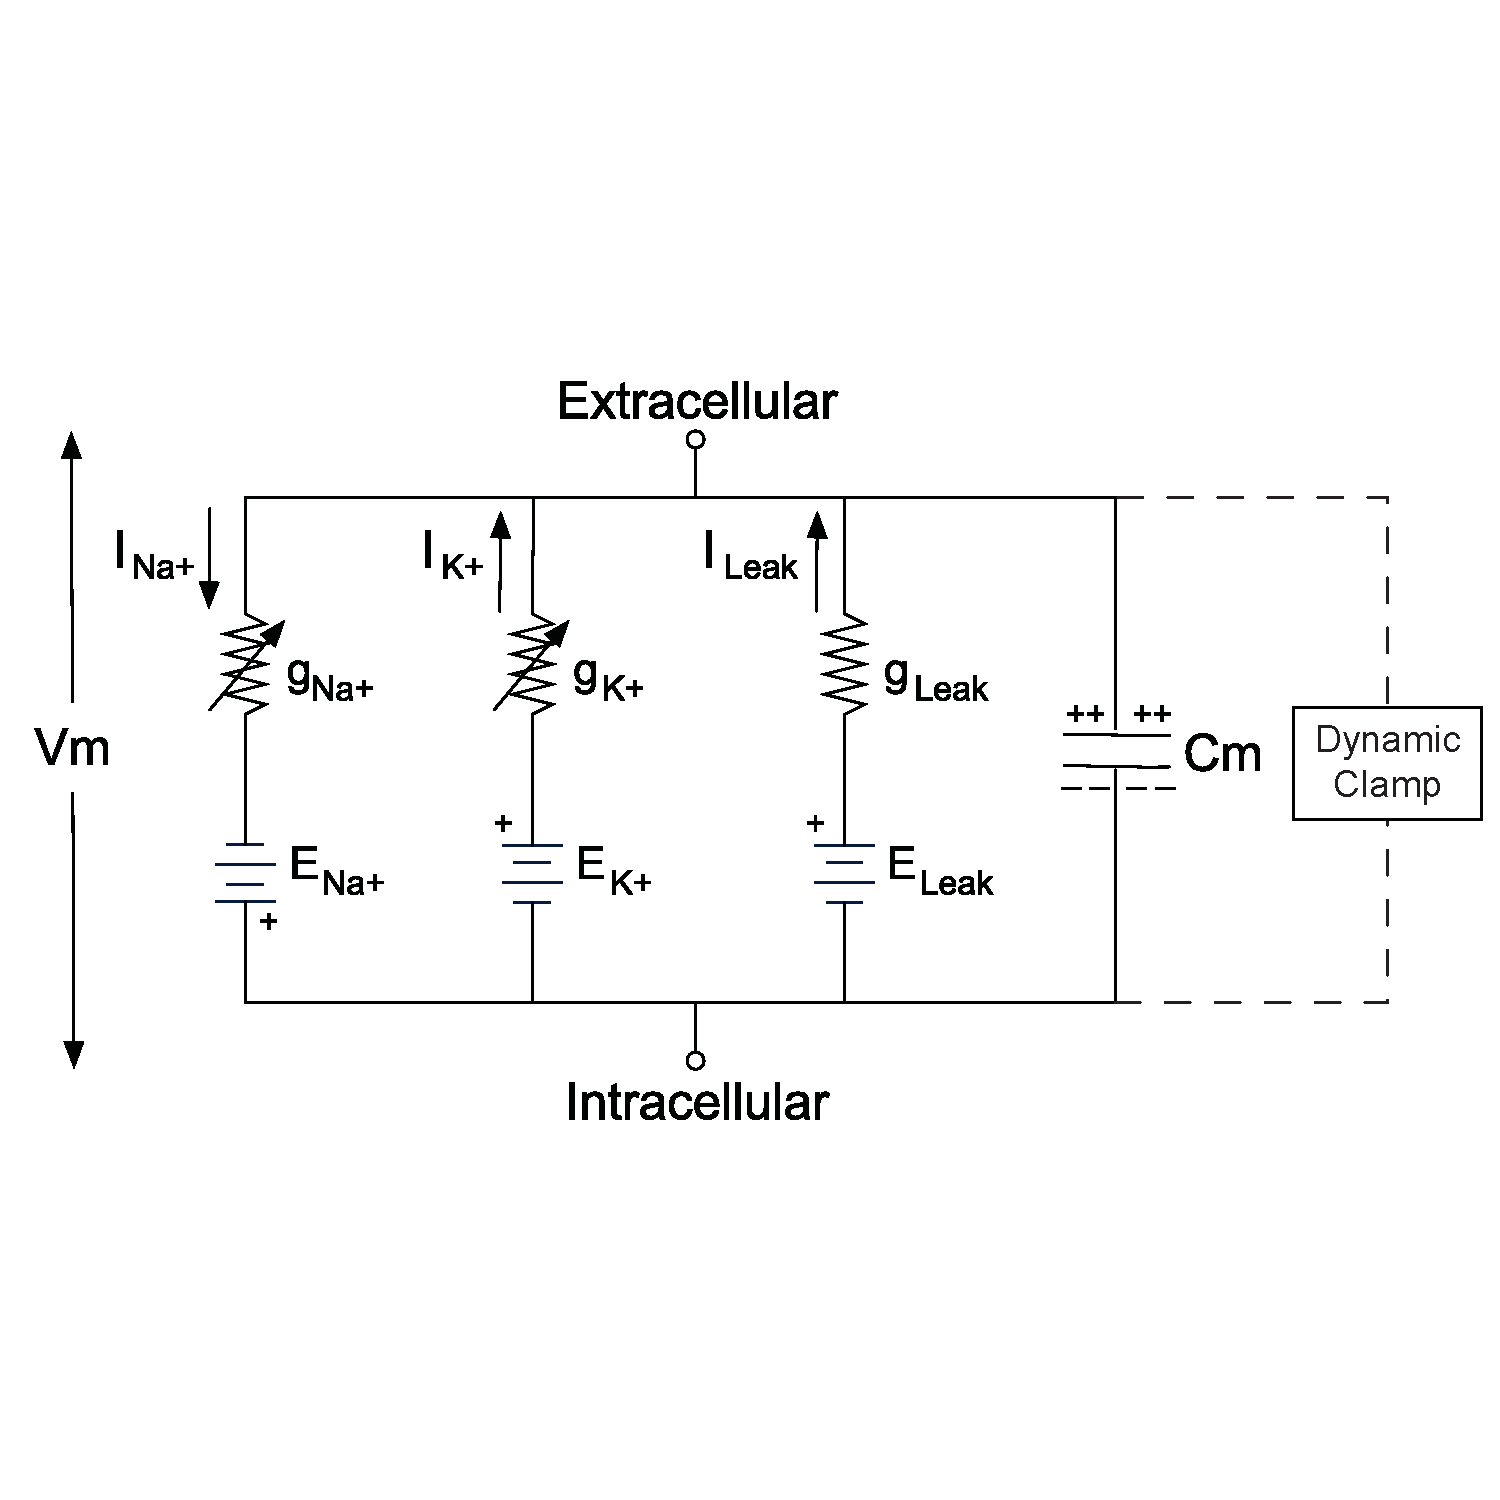
\includegraphics[width=4.5in]{dclampcircuit.pdf}
\caption[Equivalent circuit model of an excitable cell]{Equivalent circuit model of an excitable cell where $V_m$ represents the transmembrane potential, $C_m$ represents the membrane capacitance, and each conductance is defined by a reversal potential $E_{i}$ and a conductance $g_{i}$. In this model, the voltage-dependent sodium and potassium ion channels are depicted as variable resistors where $g_{i}=g_{i}(V_{m})$ . The reversal potential (or equilibrium potential) of an ion is the value of transmembrane voltage at which diffusive and electrical forces counterbalance, so that there is no net ion flow across the membrane. The reversal potential is represented as a battery since the potential difference $V_{\textrm{m}}-E_{i}$ gives the driving force across the membrane for that ionic current.} 
\label{fig:circuit} 
\end{center}
\end{figure}

The total transmembrane current is related to changes in the membrane potential, $V_{m}$, through the following equation: \index{neuron model}
\begin{eqnarray}
C_{m} \frac{dV_{m}}{dt} =-\Sigma I_{i}
\end{eqnarray}
where $C_{m}$ is the membrane capacitance. Any conductance that can be described mathematically can be applied to a neuron using the dynamic clamp. The current passing through an ion channel, for example, is often described by Ohm's law using the following conductance-based equation: 
\begin{eqnarray}\index{ion channel model}
I_{i} & = & g_{i}(V_{m})(V_{m}-E_{i}) \\
g_{i}(V_{m}) & = & \bar{g}_{i}m^{\textrm{p}}h^{\textrm{q}} 
\end{eqnarray}
where $\bar{g}$ is the maximal conductance, and $m$ and $h$ are voltage-dependent activation and inactivation gating variables ($p$ and $q$ are integers) that describe the kinetic activation of the channel. Gating variables have values between 0 and 1 to scale the channel conductance and are typically described by a first order differential equation:
\begin{eqnarray}
\frac{dx}{dt} & = & \frac{x_{\infty}(V_{m})-x}{\tau (V_{m})} 
\end{eqnarray}
The membrane potential is re-sampled and the equations are re-evaluated on every computational cycle of the dynamic clamp system. As such, the dynamic clamp is also sometimes termed \textit{conductance clamp} or \textit{conductance injection}. 

While the dynamic clamp was first demonstrated in cardiac electrophysiology to electrically couple embryonic chick myocytes \cite{Wilders:2006p930}, the technique was independently introduced \cite{Robinson:1993p1193,Sharp:1993p983} and is now more prevalent in neural electrophysiology \cite{Economo:2010p1795,Prinz:2004p985,Goaillard:2006p1175}. Applications of this technique include the insertion of non-native ion channels (a virtual ``knock-in''), subtraction of native ion channels (a virtual ``knock-out"), and simulation of synapses and electrical gap junctions to create small networks of biological and/or simulated neurons. By varying the parameter values of a model channel or synapse, experiments can be conducted to determine how these properties shape membrane dynamics and neuron activity. These approaches have made the dynamic clamp a valuable tool for studying the intrinsic properties of single neurons and the behavior of small neural networks. 

Dynamic clamp studies have also made important contributions to our understanding of neuronal dynamics under in vivo-like conditions in which neurons receive a constant barrage of synaptic inputs which can easily reach thousands of events per second. Artificial synaptic input can be constructed from pre-recorded activity of presynaptic neurons but is more commonly based on statistical descriptions of noisy conductance waveforms. This high conductance state has been shown to enhance the cell's responsiveness to small inputs, also known as its gain \cite{Chance:2002p1075,Destexhe:2003p1021,Sceniak:2010p1258}, and can change the signal integration of synaptic input, creating distinct modes of firing patterns \cite{Wolfart:2005p1138,Steriade:2001p4667,Rudolph:2003p4555,Destexhe:2001p1044}. The statistics of current-based versus conductance-based input, such as correlations and relative balance between excitation and inhibition, are translated differently into output statistics such as the membrane potential distribution, the distribution of interspike intervals (ISIs), the coefficient of variation (CV), and the mean and variance of the neuron's output firing rate \cite{Tiesinga:2000p1134,Rudolph:2003p4554,Kumar:2008p4586,Salinas:2000p4826}. Together, these factors result in a dynamical behavior of the neuron that is usually quite different from the intrinsic dynamics of the voltage-gated currents. 

Results from dynamic clamp experiments must be carefully interpreted due to several experimental limitations. Space-clamp problems arise in that the injected current is limited to a space around the recording electrode. In some experimental studies, an artificial dendrite is modeled as well to simulate the cable effects of synaptic inputs propagating to the action potential initiation zone \cite{Hughes:2008p993}. Since current can usually only be injected at the soma, the dynamic clamp may be a poor approximation of dendritic input in some cell types. In most cells, the dynamic clamp is operated in discontinuous current clamp (DCC) mode in which a single electrode switches between recording and current injection states. In this configuration, it is not possible to inject large conductances that approach the magnitude of the cell's intrinsic resting conductance while still accurately recording the membrane potential. The injected current induces a voltage drop through the electrode and causes measurement accuracies that are propagated through the closed feedback loop in the dynamic clamp system and may cause ringing artifacts in the recording \cite{Brizzi:2004p935,Jaeger:1999p1094,Preyer:2007p359,Preyer:2009p1228}. In larger cells, two electrodes may be used, one to record and one to inject current. Researchers also typically use the same ion channel or synapse model parameters for all cells used in an experiment, assuming that neurons of the same cell type have identical intrinsic properties, both within an animal and between animals \cite{Golowasch:2002p5763}. There usually is not time during an experiment to manually adjust the model to optimal parameters for each cell.

Compared to other real-time closed-loop experimental protocols, the dynamic clamp has perhaps the most stringent performance requirements. These limitations involve numerical, algorithmic, and hardware platform-specific issues. Dynamic clamp performance depends on how accurately the model is solved, measurement error in sampling the voltage, and the sampling rate of the system. \index{sampling rate}The sampling rate determines how much time is in a given computational cycle for various operations to be performed, and the duration of the cycle restricts the types of numerical methods that may be used to integrate the gating variables. Thus, the computational performance of dynamic clamp suffers from a trade-off between the speed of computation and numerical accuracy. Dynamic clamp sampling rates are currently chosen based on the limits of the hardware platform being used and the temporal dynamics being simulated. While it is possible to compute the time step necessary for the Euler and exponential Euler methods to achieve a desired one-step integration accuracy for a known voltage measurement error, few studies employ this technique \cite{Butera:2004p1073}. In simulations of dynamic clamp, Euler integration was insufficient to model fast sodium Na$_{v}$ channels at sampling rates under 30 kHz and nearly identical integration results for three different deterministic integration methods was only achieved at rates $\geq$50 kHz \cite{Milescu:2008p1216}. Standard performance benchmarks are needed for dynamic clamp to justify the sampling rates that are used.

Other hardware that are typically required for dynamic clamp are an electrophysiology amplifier for measuring membrane potential and injecting current and a multifunctional data acquisition system (DAQ) for performing analog-to-digital (ADC) and digital-to-analog (DAC) conversion. The technical specifications of each of these hardware components can affect the performance of the overall system by introducing additional jitter, latency, and quantization error that can affect system timing and the numerical computation \cite{Bettencourt:2008p1114, Butera:2001p910}. Recent results show that faster systems would result in a greater range of conductances that could be utilized, improved stability, and more accurate real-time model simulations \cite{Preyer:2007p359,Preyer:2009p1228}. Faster dynamic clamp systems have been developed, largely due to the increasing power of personal computers, but also due to the development of systems based on the GNU/Linux operating system and embedded real-time processors. 
 
 
%%%%%%%%%%%%%%%%%%%%%%%%%%%%%%%%%%%%%%%%%%%%%%%%%%%%%%%%%%%%

\chapter{RTXI Features}

\marginlabel{Hard real-time platform}RTXI provides a platform for data acquisition and custom control paradigms involving a variety of hardware and software algorithms. It runs on a hard real-time Linux operating system (OS), which guarantees reliable timing for periodic tasks such as sampling from experimental equipment, performing computations, and generating external signals. This differs from platforms based on general purpose operating systems that assign different scheduling priorities to tasks based on optimizing the user experience in a multitasking environment. For closed-loop applications such as dynamic clamp that run at very high sampling rates, it is important that data is sampled at a precise time and that all computations are completed in time for the next scheduled feedback input. Operating systems that can absolutely guarantee a maximum time for these operations are referred to as �hard real-time,� while operating systems that can only guarantee a maximum most of the time are referred to as �soft real-time.� A soft real-time system can handle such lateness, usually by pausing processes with a lower priority. For dynamic clamp, a soft real-time system may occasionally wait so long to compute the injected current, that the actual value of the membrane potential has changed in the meantime. In that case, the simulated ion channel (or other membrane conductance) is based on incorrect assumptions about the state of the system. Real-time Linux also maximizes the sampling rate that can be used by minimizing system latencies related to the hardware and analog-to-digital conversion (and vice versa). For some experimental designs with closed-loop feedback, a higher sampling rate improves the stability of the protocol.

\marginlabel{Modular architecture}Users can quickly implement complex experimental protocols in RTXI, including both open and closed-loop control modes as well as many data acquisition modes. This is accomplished by RTXI's unique architecture in which system features and custom user code are implemented as modules. Modules contain function-specific code that can be used in combination to create larger workflows. They communicate with each other within the RTXI workspace by a system of  \emph{signals and slots} and event handling. All data acquired through a DAQ card are preserved as signal streams that can be passed to other modules that implement real-time analyses such as event detection, digital filters, etc. Similarly, all user modules can accept input signals and generate output signals that can be connected to other modules or to a DAQ card to produce external analog or digital signals. In the following example of a RTXI workflow for a dynamic clamp protocol, the recorded membrane potential from a cell is connected to a module that contains a model of an ion channel. The output of the module is the computed current, which is based on the value of Vm. The output signal from the ion channel module is connected to the DAQ card so that it can be injected back into the cell. The Oscillocope can plot any signal in the workspace, including actual outputs of a model as well as internally computed state variables.

\begin{figure}[h!]
\begin{maxipage}
\begin{center}
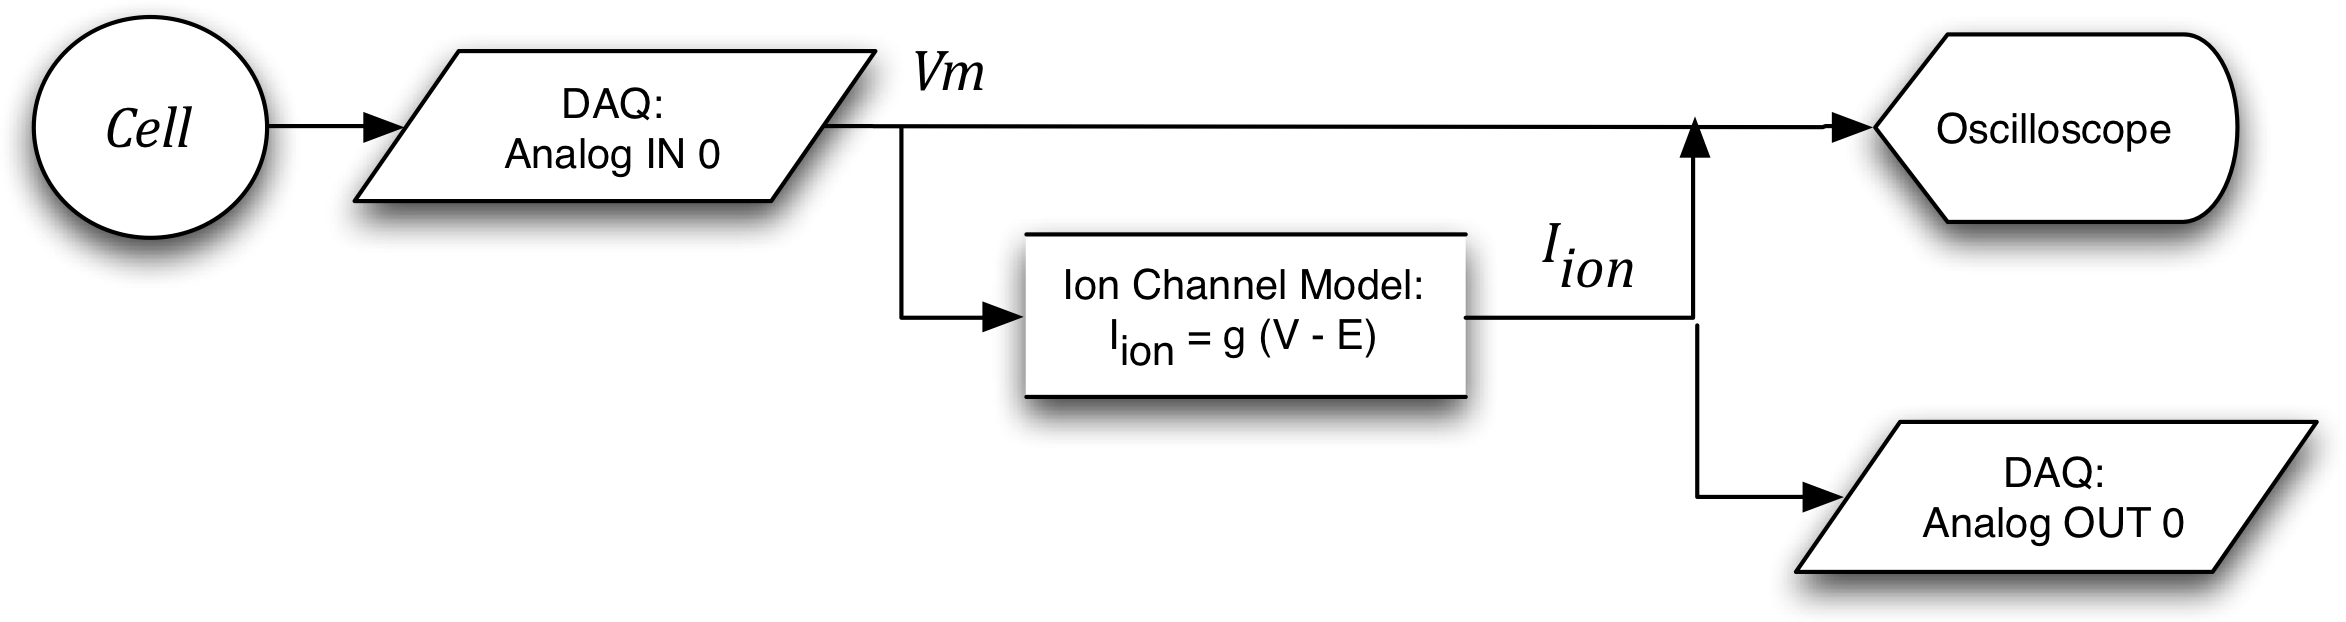
\includegraphics[width=6in]{module_ex1.png} 
\caption[RTXI Workflow Example 1]{A user module computes a current based on a model of an ion channel and the acquired value of the cell's membrane potential.} 
\label{fig:Workflow 1}
\end{center}
\end{maxipage}
\end{figure}

This modular signal-and-slots architecture allows multiple instantiations of user modules and all modules accept one-to-many and many-to-one connections. For example, a single module output signal can be routed to multiple targets. If multiple signals are connected to a single target, or slot, the signals are summed before being used in any further calculations within the module. This framework makes it easy to reuse code and implement branching logic. It is similar to graphical programming frameworks used in MATLAB\tm Simulink$^{\textrm{\textregistered}}$ and LabVIEW\tm. In the following example, a biological cell is reciprocally coupled through artificial synapses to a model neuron simulated within RTXI. The synapse is triggered by a presynaptic action potential and the synaptic current is modeled using a conductance-based equation that also depends on the measured membrane potential of the presynaptic neuron. In Figure \ref{fig: Workflow 2}, the membrane potential is split into two streams. One is sent to a Spike Detector module, which generates a trigger signal for the Synapse Model module. The other branch is sent directly to the Synapse Model module to be used in the calculation of the synaptic current. Each of these modules is instantiated twice since the two neurons are reciprocally coupled. Furthermore, each instantiation operates completely independently and can have different parameter values. This modular approach makes it very easy to experiment with asymmetric coupling, where one synapse is stronger than the other, by using different values for the maximal conductance or the reversal potential of the synapse.

This modular architecture also allows RTXI to be used solely as a experimental control system or as both a control system and data acquisition system. RTXI can be installed on most personal desktop and laptop computers and it is possible to run RTXI without a data acquisition card. This allows users to develop modules and online algorithms on one computer and copy their module to the actual computer used for experiments.

\begin{figure}[h!]
\begin{maxipage}
\begin{center}
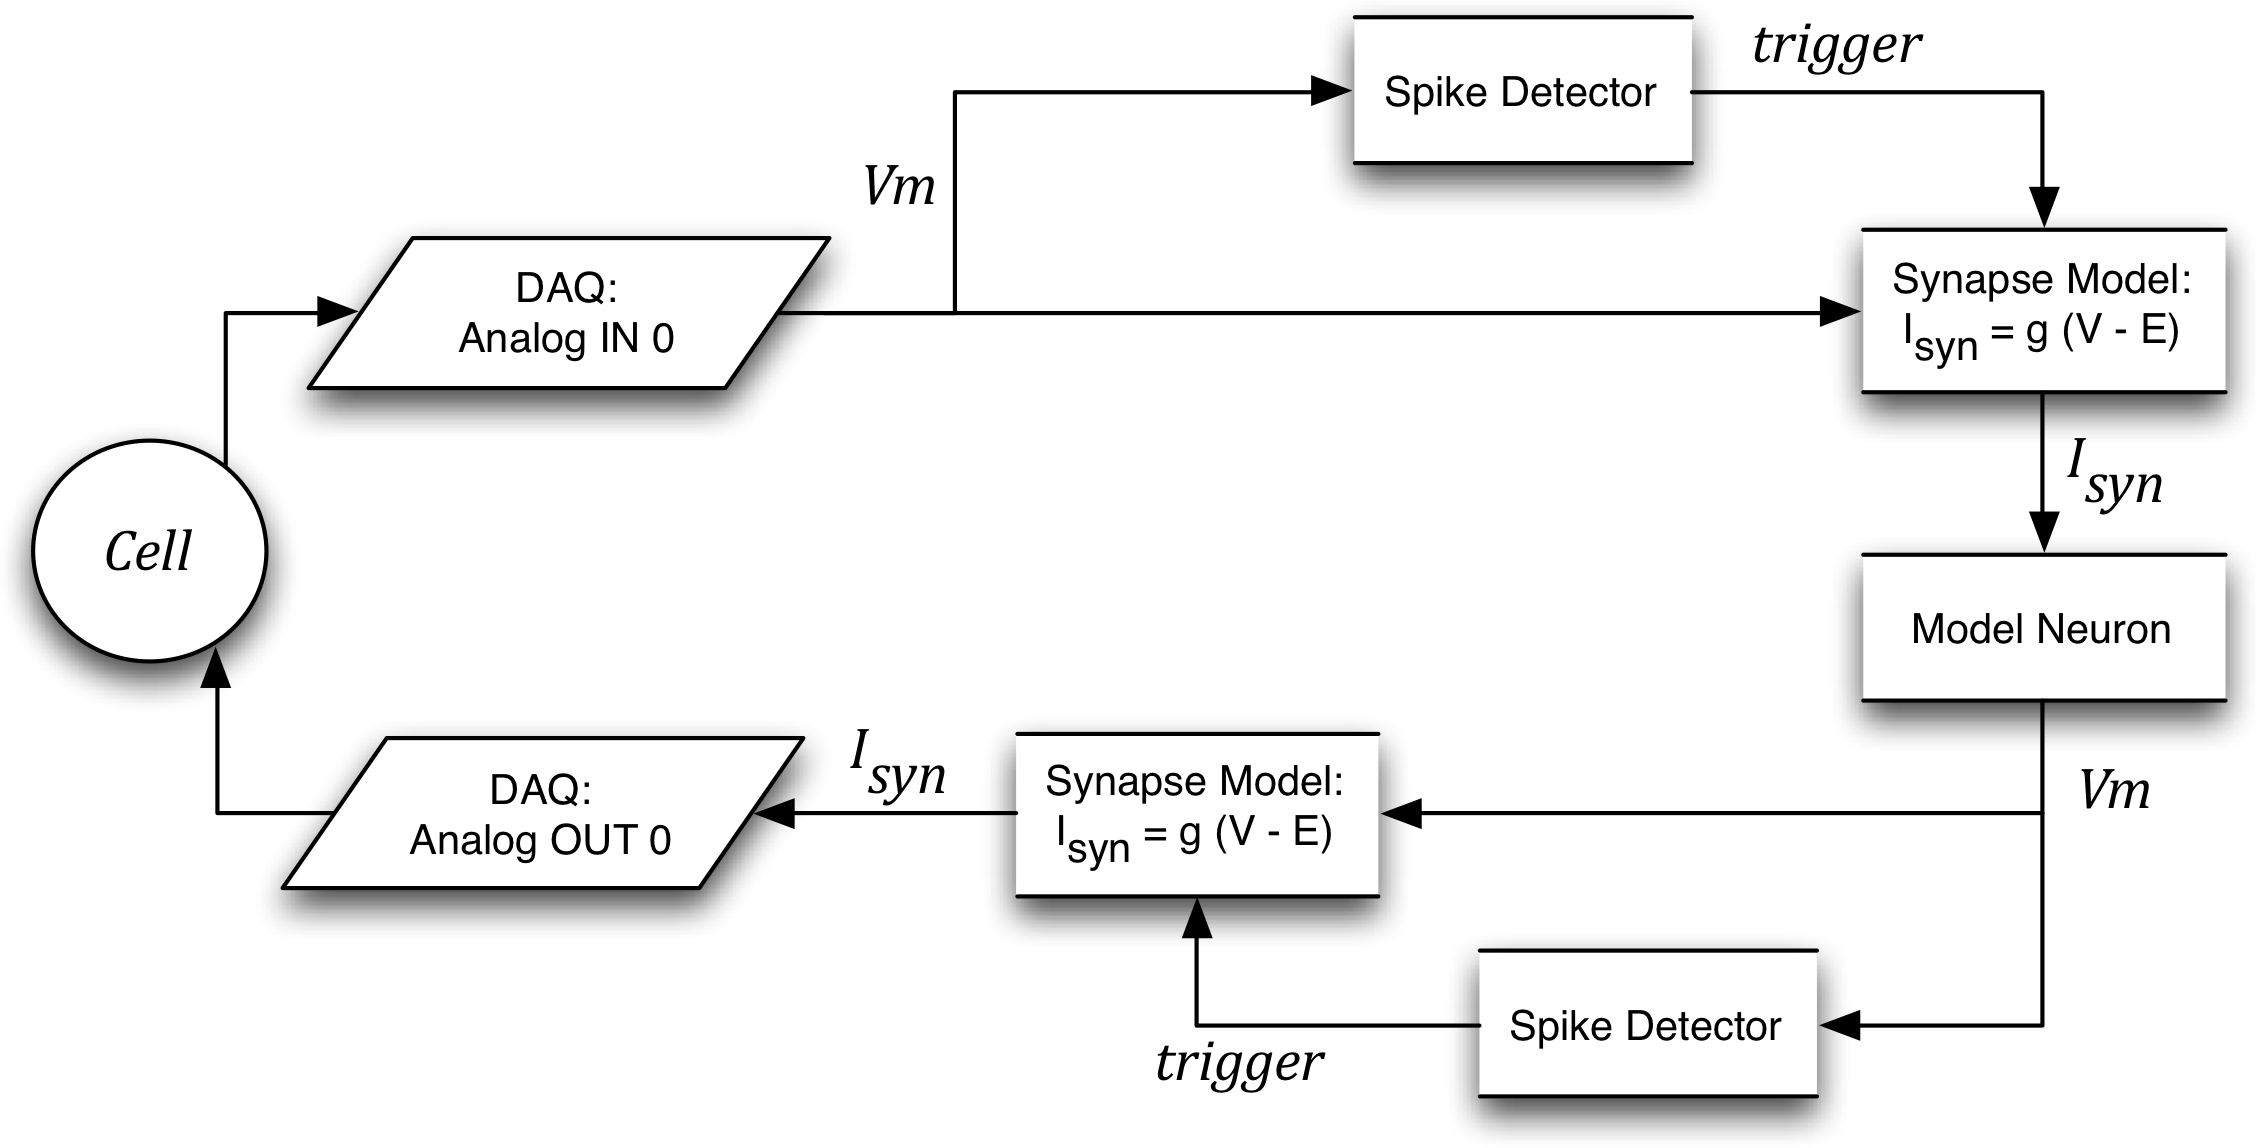
\includegraphics[width=6in]{module_ex2.png} 
\caption[RTXI Workflow Example 2]{Two user modules, a Spike Detector and a Synapse Model, are used to reciprocally couple a biological neuron with a model neuron. Each module is instantiated twice and can have different parameter values.} 
\label{fig: Workflow 2}
\end{center}
\end{maxipage}
\end{figure}

\marginlabel{Changing parameters on-the-fly} If you choose to change modules during an experiment, e.g. to change spike detection algorithms or use a different synaptic model, it is as simple as loading the new module and adding the connections. Other popular platforms for real-time closed-loop data acquisition may require you to recompile your program or re-download it onto a dedicated real-time processor. Similarly, an important feature of RTXI is the ability to change experimental parameters on-the-fly without recompiling or stopping real-time execution. This is accomplished through an intuitive GUI interface.

\marginlabel{Custom algorithms}RTXI and all core system features are written in \cpp and are based on the Qt GUI framework. Users implement custom experimental protocols by \seealso{Chapter \ref{custommodules}\\Custom User Modules}writing their own modules, in either \cpp or the DYNAMO scripting language. User-contributed modules are available on the website (http://www.rtxi.org) and examples are included in the RTXI source code. There is virtually no limit to what can be implemented in RTXI. Users can link to \cpp libraries of their own or that others have created to leverage complex computations or algorithms. Custom protocols can include not only unique online or real-time analysis but also unique experimental \emph{control} paradigms. Examples include the automation of protocols by automatically changing parameter values or using event detection to trigger a new sequence of experimental perturbations. 

The flexibility of RTXI through custom \cpp modules gives it features that are not common to other data acquisition systems, especially those for electrophysiology experiments. For example, RTXI is a complete simulation platform that can be used to solve systems of differential equations in real-time and integrate biological signals acquired in real-time with model systems. This was demonstrated in Figure \ref{Workflow 2}. Modules can also be written to load data from external files. RTXI has the ability to ``play back" this previously acquired data or surrogate data as if it were being acquired in real-time. This is accomplished by using a module that generates an output signal based on this surrogate data. Thus, online algorithms in development can be thoroughly tested and debugged using actual real-time execution without using the resources and time required for setting up an actual experiment. There are several advantages of this approach over simulating real-time computation offline using other platforms. First, it automatically takes into account the computing overhead associated with the actual RTXI system and gives a more accurate picture of your real-time performance. It also eliminates any redundant programming tasks involved with migrating code between platforms.

\marginlabel{Custom data acquisition}By default, RTXI runs \emph{continuous} protocols in that both the Data Recorder and digital Oscilloscopes modules act primarily as chart recorders. In addition, modules continuously execute their real-time code until they are paused. More complex sequences of operations can be accomplished by programming different operating modes within a single module. It is also possible to write a module that programmatically starts and stops other user modules. These "parent" or "controller" modules can be used to construct complex sequences or hierarchies of experimental stimuli. \emph{Sweep-based} or \emph{trial-based} recordings are implemented by a module that instructs the Data Recorder to increment trials. In addition, a module that generates a timed trigger signal can be used along with the trigger feature of the Oscilloscope to align recorded data in time. Examples of all these methods of implementing complex control paradigms are available.

\marginlabel{Metadata capture}RTXI can be used in parallel with your choice of data acquisition software. However, RTXI's ability to capture important metadata about an experiment is only present if it is also used for data acquisition. This is accomplished through the Data Recorder system module which streams the acquired data along with any computed signal to a Hierarchical Data Format (HDF5) file. HDF5 is an open data model that is increasingly popular for representing complex data, data relationships, and their associated metadata. In RTXI, any module that generates data that is being saved to HDF5 also has its parameters and parameter values stored in the same file. This includes not only acquired data, but also any computed intermediate signal, which is valuable for debugging algorithms offline. When a parameter value is modified on-the-fly during data acquisition, the new value and a timestamp for the modification is also saved. Other system parameters are also automatically saved to the HDF5 file so that important metadata is always adjacent to the actual experimental data. RTXI modules also exist for explicitly saving comments or creating custom experimental logs to capture any additional information. Such user modules can be used to standardize experimental logs by providing templates for information that the user is expected to supply or a finite set of options the user can choose from.

\marginlabel{Portability}Once a protocol has been created by making connections between modules and setting parameter values, the entire workspace can be captured to a settings file. Reloading this file will restore all system and user module settings, as well as the layout of the windows on the screen. This reduces the chances of errors when setting up a complicated experiment. These settings files can be transferred between different computers as long as the target computer contains the modules that were used. This is \seealso{Chapter \ref{COMEDIsupport}\\COMEDI support}independent of the actual experimental equipment that you use for data acquisition and/or current injection. RTXI uses the open source COMEDI drivers, which provides a generic interface to your choice of hardware. Users should check that they are using the correct hardware driver and configure their channel gains such that RTXI modules are receiving values in the correct units. The settings file uses a simple XML-based syntax and can be opened in any generic text editor to manually edit the default parameter values.

\seealso{Chapter \ref{HDF5}\\HDF5}HDF5 files are also compatible with many commercial and free software for a variety of platforms. There is no required proprietary software for viewing or analyzing data stored in RTXI-generated HDF5 files. Much of the available software also support editing data in place within the HDF5 file or appending new data to an existing file. This allows users to add associated data such as images, post-processed data, or additional notes.

\section{RTXI Menus}

Although RTXI is dependent on Linux, it is a complete desktop application and configuration of system settings and interaction with most features are available through a graphical user interface.

The \textbf{File Menu} is used to save and load settings files that capture the entire working environment. This includes settings configured in the System Control Panel, such as channel gains, parameters set within modules, and connections between modules. Reloading a settings files will also restore the window sizes and positions at the time the file was created. Recently used settings files are also available from this menu.

\begin{figure}[h]
\begin{center}
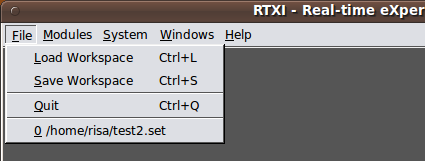
\includegraphics[width=4.5in]{fileMenu.png} 
\caption[File Menu]{The File Menu is used to save and load settings files that help you capture and recreate your working environment.} 
\end{center}
\end{figure}

The \textbf{Modules Menu} is used to load user modules or compile DYNAMO model descriptions. User modules are shared libraries that are installed to \texttt{/usr/local/lib/rtxi} during the compilation process. Choosing "Load User Module" opens a file dialog box at this location, from where users may select modules based on the *.so filename. Choosing "Load DYNAMO Model" will open a file dialog box that can be used to select a *.dynamo file containing a DYNAMO model description. This file will be parsed to generate a \cpp header and implementation file that will then be compiled to produce an RTXI module based on the \texttt{DefaultGUIModel} class. After the initial parsing and compilation, this module may then be loaded using the first menu item as with other user modules.

\begin{figure}[h]
\begin{center}
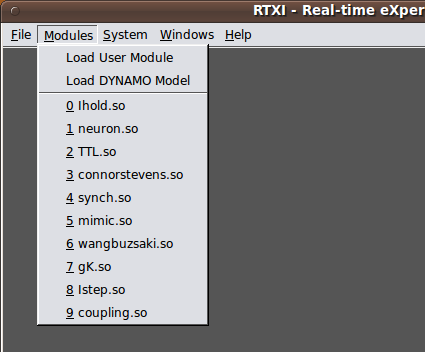
\includegraphics[width=4.5in]{modulesMenu} 
\caption[Modules Menu]{The Modules Menu is used to load user modules and compile DYNAMO models into RTXI objects.} 
\end{center}
\end{figure}

The \textbf{System Menu} is used load core RTXI system features and modules. The Control Panel is used to configure channels and set the nominal system period (or sampling rate). The Oscilloscope is the digital oscilloscope that can be used to plot any signal in real-time. The HDF Data Recorder allows users to select signals to stream to a HDF5 file in real-time. The Connector is used to specify connections between modules and the DAQ card. The Performance Measurement module displays running statistics on the computational load currently used by RTXI and how it compares to the nominal system period, or the amount of time available for performing the computations. There is also a Preferences panel for specifying commonly used directories, etc.

\begin{figure}[h]
\begin{center}
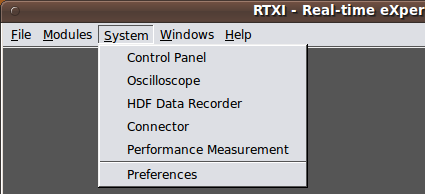
\includegraphics[width=4.5in]{systemMenu.png} 
\caption[System Menu]{The System Menu is used to access system settings and other core RTXI tools.} 
\end{center}
\end{figure}

The \textbf{Help Menu} contains important information about your system and RTXI. Choosing the "What's This" menu item turns the mouse cursor from a pointer into a question mark. In this mode, clicking on any module will display a window with contextual help, if available, about that module.

\begin{figure}[h]
\begin{center}
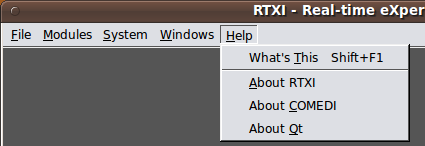
\includegraphics[width=4.5in]{helpMenu.png} 
\caption[Help Menu]{The Help Menu gives users access to contextual help for other modules and information about RTXI, COMEDI, and Qt.} 
\end{center}
\end{figure}


\section{Core System Modules}
The following modules are included in RTXI by default and are available through the \textbf{System} menu. No additional modules are necessary for acquiring data through a DAQ card and saving data to an HDF5 file.

\subsection{System Control Panel}
\label{system control panel}
\index{System Control Panel}

The System Control Panel allows you to set important parameters on all the input and output channels of your DAQ card and set the nominal real-time period of your system. RTXI automatically detects the manufacturer and board names of available DAQ cards and the number and type of input and output channels. The first DAQ card installed in your system is assigned the Linux device name: \texttt{/dev/comedi0}. \seealso{Chapter \ref{more DAQ cards}\\Configure RTXI for more cards}Additional DAQ cards are assigned device names \texttt{/dev/comedi1} and so on.

\begin{figure}[h]
\begin{center}
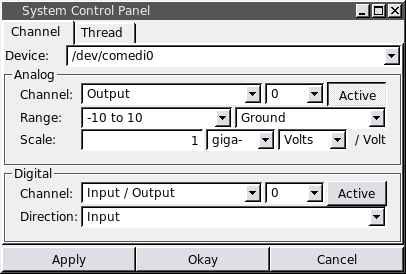
\includegraphics[width=4.5in]{systemcontrol0.png} 
\caption[System Control Panel: Channel Tab]{The Channel Tab allows users to activate and set channel properties on the DAQ card.} 
\end{center}
\label{fig:systemcontrolpanel0}
\end{figure}

\marginlabel{Channel Tab}\index{DAQ, configuration}By default, RTXI assumes that all analog DAQ input and output channels have a range from -10 V to +10 V, unity gain (or a scaling of 1 V/V), and a ground reference. You must set the correct options for each channel you are using to acquire and output the correct signal values. In the screenshot below, the DAQ card is being used as a signal generator on the first analog output channel (Channel 0). This channel is connected to an external amplifier that specifies a gain of 1 nA/V. This gain is inverted here to 1 gigaVolt/Volt to output the correct values and can be verified on an external oscilloscope. For your own reference, you could set the dropdown boxes to read 1 gigaAmp/Volt to indicate that you are ultimately generating a current signal, but this setting does not affect the computation. \attention You must click the \textbf{``Active"} toggle button to actually activate the channel. You must click \textbf{``Apply"} to commit changes made to any other channel properties such as the scale. When you have set the correct parameters for all your input and output channels, you can save your settings by choosing \textbf{File}$\rightarrow$\textbf{Save Workspace} from the RTXI menu bar. This will create a basic *.set file that you can load in the future to recreate this environment or use as a foundation for additional *.set files.

\marginlabel{Thread Tab}\index{real-time period}\index{sampling rate}In the Thread tab, you can change the real-time period of the entire system. You must click ``Apply" for this change to take effect because it triggers a real-time event that is propagated to other modules. \seealso{Chapter \ref{pause flag}\\\texttt{DefaultGUIModel} PAUSE flag}Custom user modules can be programmed to execute specific code when the system's real-time period is changed.

\begin{figure}[h]
\begin{center}
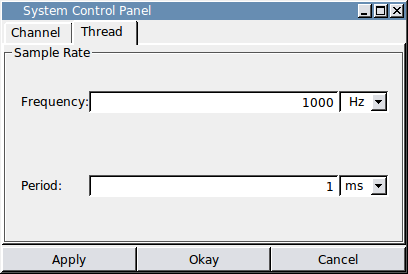
\includegraphics[width=4.5in]{systemcontrol1.png} 
\caption[System Control Panel: Thread Tab]{The Thread Tab allows users to change the period for real-time execution.} 
\end{center}
\label{fig:systemcontrolpanel1}
\end{figure}

\subsection{Oscilloscope}
\label{Oscilloscope}
\index{Oscilloscope}

The Oscilloscope allows you to plot any system signal in real-time, including signals from/to the DAQ card and signals from user modules. To plot multiple signals, you can instantiate multiple oscilloscopes or superimpose multiple signals on a single oscilloscope. Each signal may have a different vertical scale and line style and a legend is automatically generated in the Oscilloscope window. Below is a screenshot of the Oscilloscope acquiring data using the CLAMP-1U model cell (by Molecular Devices) with an applied square pulse current. It is plotting two input channels from the DAQ card as well as the command current (Iout1) generated by a module. The lower right-hand corner displays the time scale for each grid division. \attention The Oscilloscope uses a right-click context menu that allows you to pause/unpause real-time plotting or access the ``Properties" panel for choosing signals and setting the axes properties.

\begin{figure}[h]
\begin{maxipage}
\begin{center}
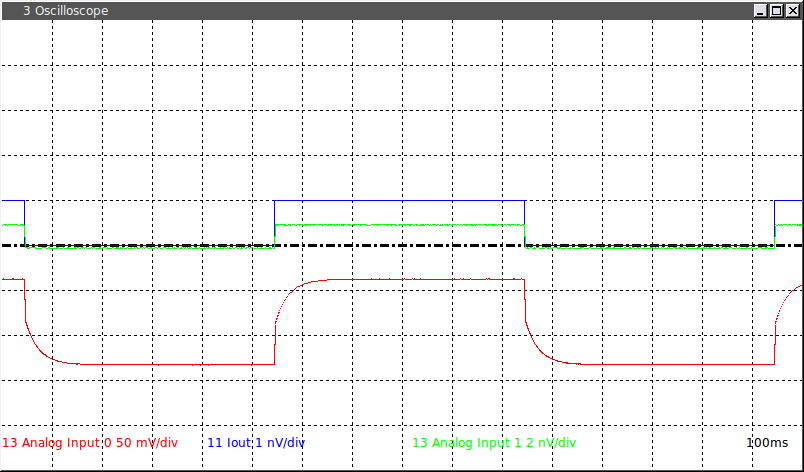
\includegraphics[width=6in]{oscilloscope0.png} 
\caption[Oscilloscope]{The Oscilloscope can plot multiple signals in real-time.} 
\end{center}
\label{fig:oscilloscopel0}
\end{maxipage}
\end{figure}

\marginlabel{Channel Tab}On the Channel tab, you can select signals to plot. Signals from the DAQ card will appear in the ``�Channel" dropdown box as a COMEDI source, eg. \texttt{/dev/comedi0}. To get correct values for your signal, you may have to set additional settings in the \seealso{Chapter \ref{system control panel}\\System Control Panel}System Control panel if you use any other instrumentation that applies a gain to your signal. Input to the DAQ card from external instrumentation, such as an external amplifier, is designated as output from the DAQ card within RTXI. RTXI will automatically detect how many input and output channels your card has. Signals from other modules will be identified by the module name and you can choose from any inputs, outputs, parameters, or states that are defined in those modules. \attention To actually plot the signal, you must depress the \textbf{``Active"} toggle button and hit \textbf{``Apply."} Any modifications you make to the scaling, offset, or line style of the signal are not active until you hit ``Apply" again. Note that plotting too many signals in real-time may affect your system performance and cause your GUI to freeze during program execution.

\begin{figure}[h]
\begin{center}
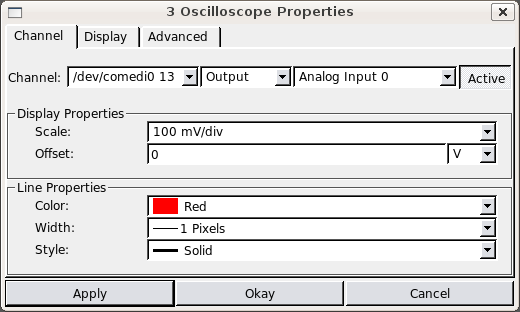
\includegraphics[width=4.5in]{oscilloscope1.png} 
\caption[Oscilloscope: Channel Tab]{The Channel Tab allows you to select the signals to plot and set line styles.} 
\end{center}
\label{fig:oscilloscope1}
\end{figure}

\newpage
\marginlabel{Display Tab}On the Display tab, you can set the time scale of the oscilloscope and the screen�s refresh rate. You can also set up a trigger to freeze the oscilloscope when certain criteria are met by the triggered channel. \index{Oscilloscope, trigger}Set the trigger to operate on a ``rising edge" or ``falling edge" by clicking the radio buttons marked ``+" or ``-", respectively. The ``Trigger Channel" can be set to any signal that is currently plotted on the oscilloscope. ``Trigger holding" allows you to set the amount of time that lapses before the trigger is reset again. The trigger threshold is indicated on the oscilloscope by a horizontal yellow dashed line.

\begin{figure}[h!]
\begin{center}
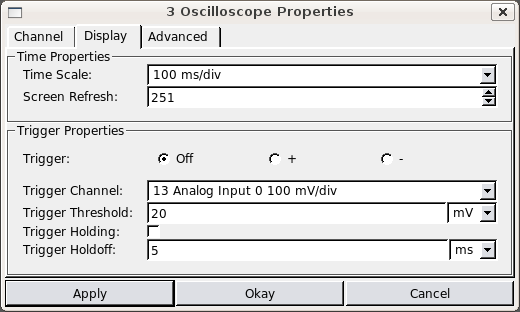
\includegraphics[width=4.5in]{oscilloscope2.png} 
\caption[Oscilloscope: Display Tab]{The Display Tab allows you to set the time scale for horizontal divisions and set a trigger on any plotted signal.} 
\end{center}
\label{fig:oscilloscope2}
\end{figure}

\newpage
\marginlabel{Advanced Tab}On the Advanced tab, you can choose to downsample the data that is plotted on the oscilloscope or change the number of grid divisions used for scaling.

\begin{figure}[h]
\begin{center}
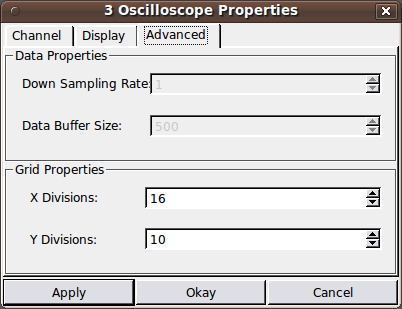
\includegraphics[width=4in]{oscilloscope3.png} 
\caption[Oscilloscope: Advanced Tab]{The Advanced Tab allows users to set downsampling rates on the plotted data, change the size of the data buffer, and change the number of divisions in the oscilloscope.} 
\end{center}
\label{fig:oscilloscope3}
\end{figure}

\subsection{Data Recorder}
\index{Data Recorder}

The Data Recorder module allows users to stream synchronous data to a HDF5 file. To record data, select \textbf{System}$\rightarrow$\textbf{Data Recorder} from the RTXI menu bar. The \textbf{``Block"} menu is a list of your DAQ card(s) and any loaded user modules. Selecting a block device then populates the \textbf{``Type"} and \textbf{``Channel"} menus. Select the Analog Input 0 channel from your DAQ device and click the \textbf{``$>$"} button. To remove a channel from the list, highlight it in the listbox and click the \textbf{``$<$"} button. Before you can start recording, you must select a file by clicking the \textbf{``Choose File"} button. Click \textbf{``Start Recording"} to begin recording and \textbf{``Stop Recording"} to stop recording. For each module connected to the Data Recorder, it also grabs all the parameters values and saves them as metadata. In addition, it logs when any of these parameter values change so that you have a complete record of your experiment. If you have a configuration such that Module A: Output 0 --$>$ Module B: Input 0, saving both of these respective signals in the Data Recorder will give you exactly the same data. Similarly, saving \texttt{/dev/comedi0}: Analog Output 0 will save the signal that has been assigned to that channel (perhaps generated by a user module), not the actual signal the DAQ card is outputting. To check the actual output of the DAQ card, you will need to make a connection from that output to another input channel.

\begin{figure}[h]
\begin{center}
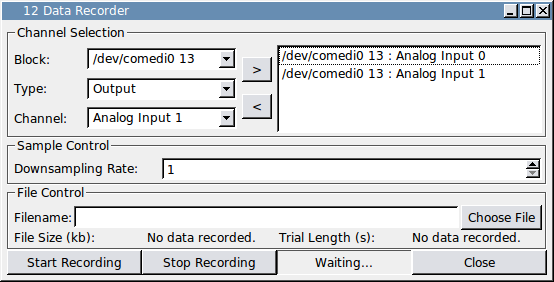
\includegraphics[width=4.5in]{datarecorder.png} 
\caption[Data Recorder]{The Data Recorder allows you to save any signal in your workspace synchronously to an HDF5 file. Use the  ``$>$" and ``$<$" buttons to add and remove signals from the list.} 
\end{center}
\label{fig:datarecorder}
\end{figure}

For real-time streaming of multiple signals, an HDF5 data type is used in RTXI that does not map efficiently onto MATLAB native data types. While MATLAB can read this data using its low-level functions, this process can be very slow. To load RTXI HDF5 files quickly into MATLAB, you will first need to run a small utility function on your HDF5 file to convert the \emph{Synchronous Data} dataset to a different data type. This function is compiled when RTXI is compiled and is located in \texttt{/rtxi/hdf}. To convert your HDF5 file:\index{rtxi\_hdf\_matlabize}
\begin{example}
\$ rtxi\_hdf\_matlablize YOUR\_FILE.h5
\end{example}

To make this utility accessible from any directory on your system, make a symbolic link in \texttt{/usr/bin} to the location of this function in your RTXI source directory. If you installed RTXI from the Live CD, the source directory is \texttt{/home/rtxi}:
\begin{example}
\$ sudo ln -s RTXI\_SRC\_DIR/hdf/rtxi\_hdf\_matlabize \\ \hspace{1cm} /usr/bin/rtxi\_hdf\_matlabize
\end{example}

RTXI also includes a simple MATLAB GUI for quickly viewing the data within a single trial. The MATLAB code is available in \texttt{/rtxi/hdf/RTXIh5}. A sample m-file is provided with examples of how to extract data to the MATLAB workspace, how to use the GUI browser, and how to add new datasets to your file. It is also possible to embed binary formats, such as images, within a trial.

\subsection{Connector}
\index{Connector}

The Connector module allows you to create connections between modules or between modules and the DAQ card. Incoming signals to RTXI through the DAQ card appear in the \textbf{``Output Block"} and outgoing signals through the DAQ appear in the \textbf{``Input Block."} RTXI automatically detects how many inputs and outputs are available for your installed DAQ card. Similarly, any signal that is defined as an output of a module appears in the ``Output Block" and any input slot of a module appears in the ``Input Block." After you have made your selection, click the central toggle button to activate the connection. Your active connections are listed in the ``Connections" box. To quickly turn off an existing connection, double-click on its entry in the table and click the toggle button. Below is a screenshot of how to connect the command current from the Istep module to the first analog output channel of the DAQ card.

\begin{figure}[h]
\begin{center}
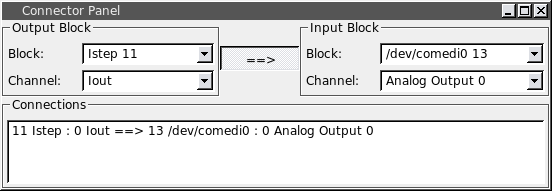
\includegraphics[width=4.5in]{connector1.png} 
\caption[Connector]{The Connector allows you to connect any signal from the left ``Output Block" and connect it to a slot in the right ``Input Block". RTXI automatically detects the available signals and slots from the DAQ card and any loaded user modules.} 
\end{center}
\label{fig:connector1}
\end{figure}

Here is a screenshot containing connections between modules only. The membrane potential of a model neuron is fed into a spike detector that in turn, informs a dynamic clamp module when spikes have occurred. The model cell�s voltage is also fed into the dynamic clamp module for computing the current that is connected back to the model cell. \attention The signals-and-slots architecture of RTXI allows any signal to be connected to any slot. In this example, the spike detector could accept input from any model neuron simulated within RTXI or input from an actual recorded cell. RTXI also allows one-to-many and many-to-one connections. If multiple signals are connected to one slot, the signals are first summed before any additional operations are performed. Thus, multiple signals could be connected to be a single output channel of your DAQ card, allowing you to ``stack" stimuli being generated from multiple user modules.

\begin{figure}[h]
\begin{center}
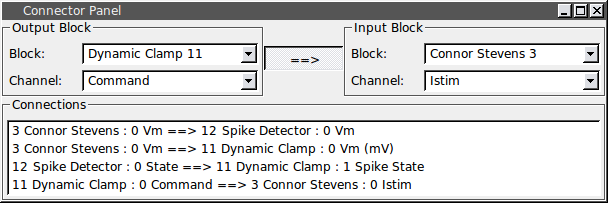
\includegraphics[width=4.5in]{connector.png} 
\caption[Connector]{The signals-and-slots architecture of RTXI allows any signal to be connected to any slot and allows one-to-many and many-to-one connections.} 
\end{center}
\label{fig:connector}
\end{figure}

\subsection{Performance Benchmark}

The Performance Benchmark module gives you timing statistics for RTXI. For hard real-time performance, it is important that all operations, computations executed by user modules and tasks related to data acquisition, etc., complete within the nominal system period. This module continuously keeps track of the time needed to complete these tasks, updated once every second in the GUI, as well as the actual real-time period. In addition, the module reports the worst case total computation time and the worst case time step since the statistics were last reset.

\begin{figure}[h]
\begin{center}
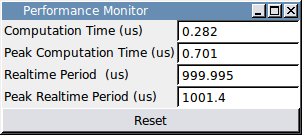
\includegraphics[width=3in]{performancebenchmark0} 
\caption[Performance Benchmark]{The Performance Benchmark module gives you timing statistics related to computational tasks and the actual real-time period (system sampling rate).} 
\end{center}
\label{fig:performancebenchmark0}
\end{figure}

%%%%%%%%%%%%%%%%%%%%%%%%%%%%%%%%%%%%%%%%%%%%%%%%%%%%%%%%%%%%%%%%%%%%

\chapter{Getting Started}

%%%%%%%%%%%%%%%%%%%%%%%%%%%%%%%%%%%%%%%%%%%%%%%%%%%%%%%%%%%%

\section{Installing User Modules}
\label{module installation} \index{modules, installation} \index{installation, modules}
RTXI comes with a limited set of core system modules and sample user modules. All modules are compiled as Linux shared object libraries that are linked into the core system. This allows RTXI to have minimal overhead and user modules are loaded only as needed. This architecture also allows multiple instantiations of user modules so that elements such as filters and event detectors can be reused on a variety of signals. 

Example user modules are available on the RTXI website (http://www.rtxi.org) as compressed tarballs (*.tar.gz extension). Each module consists of a single directory, typically containing a single class header file (*.h), class implementation file (*.cpp), and a Makefile that informs the GCC compiler. It is recommended that user modules be stored together in a single directory (such as \texttt{\$HOME/modules}). Some of the examples on the website refer to other base classes that can then be kept in a common include folder (such as \texttt{\$HOME/modules/include}). To extract a module directory and compile the module:
\begin{example}
\$ tar xvf myplugin.tar.gz\\
\$ cd myplugin\\
\$ sudo make install
\end{example}

The RTXI object library (*.so extension) will be copied to \texttt{/usr/local/lib/rtxi}, which is where RTXI will initially look for them. User modules must be recompiled if any changes are made. Users should carefully name their custom modules since the compiled binaries are automatically overwritten. \attention In RTXI versions 1.2 and later, user modules are compiled outside the RTXI source tree and the Makefile is much simpler. A slightly more complicated process is required to compile modules for earlier versions of RTXI. Instructions for writing custom user modules are given in Chapter \ref{custommodules}.

%%%%%%%%%%%%%%%%%%%%%%%%%%%%%%%%%%%%%%%%%%%%%%%%%%%%%%%%%%%%

\section{Acquiring Data (Model Cell Tutorial)}

This section presents a tutorial similar to those described by Molecular Devices for their suite of electrophysiology products. This exercise uses a CLAMP-1U model cell with an Axon\tm Axoclamp\tm 2B amplifier operating in bridge mode. Connect the HS-2A-x0.1LU headstage to the ME1 PROBE connector and the HS-2A-x1LU head stage to the ME2 probe connector on the back panel of the amplifier.

\marginlabel{Connect equipment\\to DAQ card} Make the following connections between the amplifier and the DAQ card. 
\begin{enumerate}
\item Axoclamp 10Vm Output $\rightarrow$ DAQ Analog Input 0
\item Axoclamp Im Output $\rightarrow$ DAQ Analog Input 1
\item DAQ Analog Output 0 $\rightarrow$ Axoclamp EXT. ME1 COMMAND
\end{enumerate}

\marginlabel{Start RTXI} If you have not already calibrated your DAQ card, use \texttt{comedi\_calibrate} or \texttt{comedi\_soft\_calibrate} (if you have an NI M-series card):
\begin{example}
\$ sudo comedi\_calibrate --reset --dump --calibrate --results --verbose /dev/comedi0
\end{example}
If you installed RTXI using the Live CD, you may start RTXI from the Applications menu. However, it is a good idea to start RTXI from the terminal since some modules output error messages or warnings to the terminal: 
\begin{example}
\$ rtxi
\end{example}
\vspace{1cm}
\marginlabel{Configure DAQ Channels} \index{DAQ, configuration}While RTXI automatically detects the available channels on your DAQ card, they need to be configured inside RTXI. From the \textbf{System} menu on the RTXI menu bar, choose the \textbf{Control Panel}. The default device should be your DAQ card listed as \texttt{/dev/comedi0}. The analog channels on most multifunction DAQ cards have a range of -10 V to +10 V based on a ground reference and this is the default in RTXI. You should check the specifications for your DAQ card and choose the corresponding settings in RTXI. For Analog Input 0, the amplifier specifies that the signal has a gain of 10 applied (10Vm). Invert this and enter a scale of 0.1 V/V for this channel. Click the \textbf{``Active"} toggle button and click the \textbf{``Apply"} button. You will not acquire any actual data on a channel until it has been set to ``Active."
\begin{figure}[h]
\begin{center}
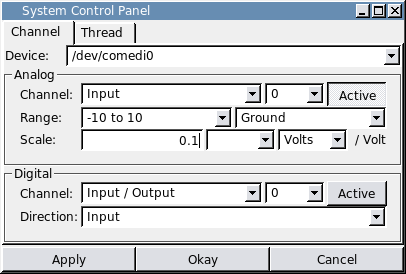
\includegraphics[width=4in]{axoclamptutorial0.png} 
\caption[Axoclamp Tutorial: Analog Input 0]{Configuring Axoclamp 10Vm output on Analog Input 0} 
\end{center}
\label{fig:axoclamptutorial0}
\end{figure}

\newpage For the membrane current assigned to Analog Input 1, the Axoclamp amplifier specifies that there is a gain of 10 $\div$ H mV/nA. Since the headstage gain on ME1 is H=0.1, the conversion is 100 mV/nA or 0.1 V/nA. Invert this to get a scale of 10 nA/V. You may set the ``Scale" dropdown box to either units of volts or amperes but this does not affect the computation. \attention Note that you must compute the total gain applied to a channel by any combination of hardware and software along the path of the signal. For example, if you are using the Axon\tm Multiclamp\tm Microelectrode Amplifier by Molecular Devices, you should take into account Multiclamp Commander software gain.

\begin{figure}[h]
\begin{center}
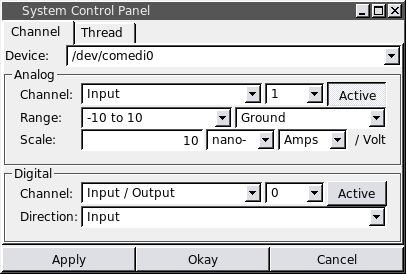
\includegraphics[width=4in]{axoclamptutorial1.png} 
\caption[Axoclamp Tutorial: Analog Input 1]{Configuring Axoclamp Im output on Analog Input 1} 
\end{center}
\label{fig:axoclamptutorial1}
\end{figure}
\vspace{1.5cm}

For the EXT. ME1 COMMAND assigned to Analog Output 0, the Axoclamp specified a gain of 10 x H nA/V, which comes to 1 nA/V. Invert this to get a scale of 1 gigaV/A.

\begin{figure}[h]
\begin{center}
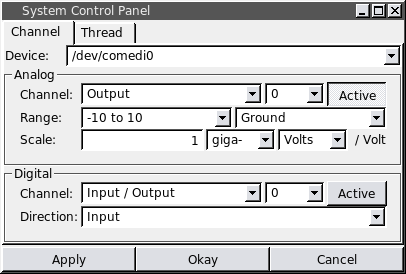
\includegraphics[width=4in]{axoclamptutorial2.png} 
\caption[Axoclamp Tutorial: Analog Output 0]{Configuring EXT. ME1 COMMAND on Analog Output 0}
\end{center}
\label{fig:axoclamptutorial2}
\end{figure}

\attention The Thread Tab of the System Control Panel allows you to set the real-time period or sampling rate \index{sampling rate} of the system. The default sampling rate is 1 kHz, which is sufficient for this exercise.

\vspace{1cm}
\marginlabel{Configure stimulus module} The Istep module generates  current step stimuli (square wave pulses). Install the Istep module according to the directions in Chapter \ref{module installation} and load it by selecting \textbf{Modules}$\rightarrow$\textbf{Load Modules} from the RTXI menu bar. Set the amplitude of the current pulse to 5 nA and set the width of the pulse to 40 ms using the Period and Duty Cycle options. The number of pulses is set using the Cycles option.

\begin{figure}[h]
\begin{center}
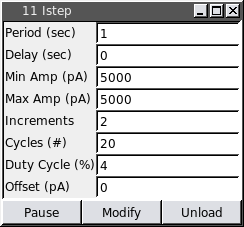
\includegraphics[width=2.2in]{istep.png} 
\caption[Istep]{The Istep module delivers current step pulses.} 
\end{center}
\label{fig:istep}
\end{figure}

\vspace{1cm}
\marginlabel{Configure Oscilloscope}Start the Oscilloscope by selecting \textbf{System}$\rightarrow$\textbf{Oscilloscope} from the RTXI menu bar. Right click anywhere in the Oscilloscope window to bring up the context menu and select the \textbf{Properties} menu. \seealso{Chapter \ref{Oscilloscope}\\Oscilloscope}The \textbf{Channel Tab} is used to select signals to plot and set an appropriate scale and line style. The architecture of RTXI is based on modular components that have input and output signals. \attention The DAQ card is abstracted as a DAQ device block such that a signal acquired on an input channel of the DAQ \emph{card} becomes an output signal of the DAQ \emph{device} within RTXI. To plot the voltage acquired on Analog Input 0, use the dropdown box to select \textbf{``Output"}. The rightmost dropdown box will automatically be populated with the analog input channels of the DAQ card. Click the \textbf{``Active"} toggle button to plot the signal. 

\begin{figure}[h]
\begin{center}
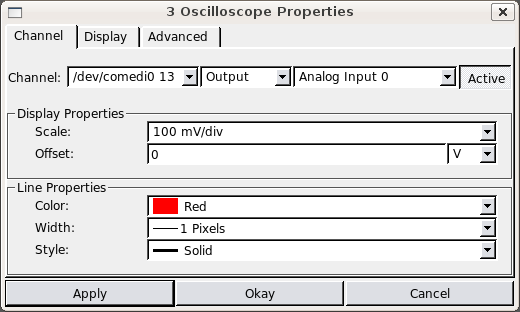
\includegraphics[width=4.5in]{oscilloscope1.png} 
\caption[Oscilloscope]{The Oscilloscope Channel Tab allows you to select signals to plot and choose different scales and line styles.} 
\end{center}
\end{figure}

When a signal is plotted, the Oscilloscope will generate a legend in the lower part of the window. In the \textbf{Display Properties} section, choose a scale and if needed, an offset. You may also choose a linestyle in the \textbf{Line Properties} section. You must click the \textbf{Apply} button for these changes to take effect. Each signal may have a different scale and different line style. Use the System Control Panel to plot Analog Input 0 and Analog Input 1 to monitor the voltage and the current applied to the model cell. You should also plot the ``Iout" output signal of the Istep module.

\vspace{1cm}
\marginlabel{Connect Signals\\Within RTXI}To generate signals from the Istep module, untoggle the \textbf{``Pause"} button. RTXI will begin executing the real-time code specified in this module. You should see pulses in the Istep signal in the Oscilloscope window. You can use the textboxes in the GUI to change the parameter values. The text will turn red but there will be no change in the module's output signal until you click the \textbf{``Modify"} button. Clicking this button initiates an event that will update the parameter in real-time and you should see the corresponding change immediately in the Oscilloscope. At this point, you  should not see any pulses in Analog Input 1 from your DAQ card, which is the current actually delivered by the amplifier. To apply this stimulus to the model cell, you need to make a connection between the Istep module and the DAQ card. From the RTXI menu bar, select \textbf{System}$\rightarrow$\textbf{Connector}. 

\begin{figure}[h]
\begin{center}
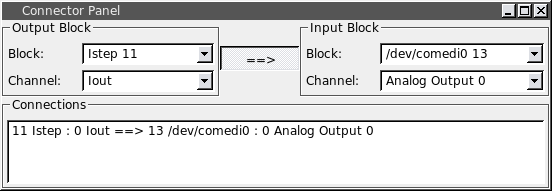
\includegraphics[width=4.5in]{connector1.png} 
\caption[Connector]{The Connector allows you to create connections between user modules or between modules and the DAQ card.} 
\end{center}
\end{figure}

The Connector module populates the \textbf{``Output Block"} with the available signals in your workspace and the \textbf{``Input Block"} with the available slots, or destinations. Select the Istep module in the ``Output Block" and the ``Iout" signal. Choose your DAQ card (\texttt{/dev/comedi0}) in the ``Input Block" and the Analog Output 0 channel. To make the connection, click the central ``==$>$" toggle button. Now, the Oscilloscope should show matching data for both Istep: Iout and Analog Input 1.

\vspace{1cm}
\marginlabel{Balance the Bridge\\ in the Bath}
Switch the CLAMP-1U model cell to the BATH position. Use the amplifier INPUT OFFSET knob to zero out the voltage based on the readings in the Oscilloscope. The Oscilloscope shows the actual sample values (with the channel gain applied) that will later be saved using the Data Recorder module. If your amplifier or other control software indicates a nonzero voltage when RTXI reports a zero voltage, \seealso{Chapter \ref{comedi calibration}\\COMEDI calibration}calibrating your DAQ card may eliminate this offset. Unpause the Istep module to begin delivering current pulses to the model cell. Adjust the BRIDGE knob until the voltage deflection is eliminated and then adjust the CAPACITANCE NEUTRALIZATION knob until the residual transients are minimized. Now switch the model cell to the CELL position. If you have correctly tuned these settings, you should see a response to each current pulse as in Figure \ref{balancedbridge}.

\begin{figure}[h!]
\begin{maxipage}
\begin{center}
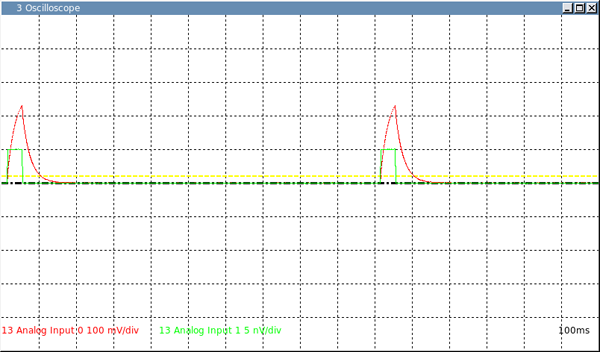
\includegraphics[width=5.2in]{axoclamptutorial3.png} 
\caption[Axoclamp Tutorial: Balanced Bridge]{Model cell response to current injection pulses with correctly balanced bridge and capacitance neutralization}
\label{fig:balancedbridge}
\end{center}
\end{maxipage}
\end{figure}

\begin{figure}[h!]
\begin{maxipage}
\begin{center}
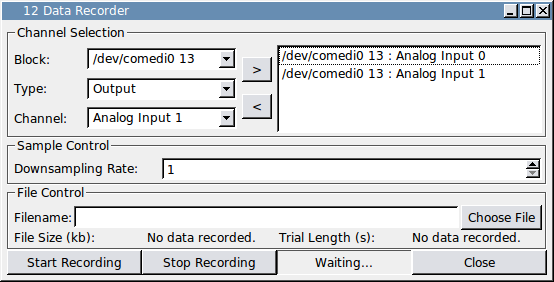
\includegraphics[width=5in]{axoclamptutorial4.png} 
\caption[Data Recorder]{The Data Recorder saves any synchronous signal in your workspace to an HDF5 file.} 
\end{center}
\end{maxipage}
\end{figure}

\marginlabel{Saving Data}To record data, select \textbf{System}$\rightarrow$\textbf{Data Recorder} from the RTXI menu bar. The \textbf{``Block"} menu is a list of your DAQ card(s) and any loaded user modules. Selecting a block device then populates the \textbf{``Type"} and \textbf{``Channel"} menus. Select the Analog Input 0 channel from your DAQ device and click the \textbf{``$>$"} button. To remove a channel from the list, highlight it in the listbox and click the \textbf{``$<$"} button. Before you can start recording, you must select a file by clicking the \textbf{``Choose File"} button. Click \textbf{``Start Recording"} to begin recording and \textbf{``Stop Recording"} to stop recording.

\vspace{1cm}
\marginlabel{Saving Your Workspace}
At this point, you have configured several channels on the DAQ card and the Oscilloscope, set custom parameters for a user module, and connected the module to the DAQ card to generate an external signal. RTXI allows you to save all these settings to a file by selecting \textbf{File}$\rightarrow$\textbf{Save Workspace} from the RTXI menu bar. To reload the file and reconstruct your entire working environment, select   \textbf{File}$\rightarrow$\textbf{Load Workspace}.

%%%%%%%%%%%%%%%%%%%%%%%%%%%%%%%%%%%%%%%%%%%%%%%%%%%%%%%%%%%%

\section{HDF5 Data Files}
\label{HDF5}\index{HDF5, file format}
The HDF5 file format is a portable and extensible binary data format designed for complex data. It features support for an unlimited variety of datatypes, and has flexible and efficient data retrieval and storage methods. HDF5 features a hierarchical structure that allows you to access chunks of data without loading the entire file into memory. An HDF5 file produced by RTXI's Data Recorder is organized as shown in Figure \ref{HDF5 structure}. 

At the topmost level, an RTXI HDF5 file is divided into separate \emph{Trial} groups, each of which contains the system settings and module parameter values that existed at the time that data was recorded. The Data Recorder only saves \attention parameters values for modules from which it is recording a signal. A new \emph{Trial} is created whenever the Data Recorder is used to start recording. For example, if you stop and start recording multiple times in a single session, RTXI automatically increments the trial number each time. If you choose to save data to a file that already exists, RTXI will prompt you with a choice to overwrite the file or append new data to the file. Appending data to a file also creates a new \emph{Trial}. Thus, it is possible to have trials within the same file that contain different parameter settings and even data downsampling rates.

Parameter values from user modules are saved in the \emph{Parameters} group within each \emph{Trial}. The name of each parameter includes the module instance ID number within RTXI, the name of the module, and the name of the parameter itself. If the value of the parameter changes during recording, all the values are saved with a corresponding index value that is the timestamp in nanoseconds from the start of the recording. This feature is only available for user modules that are \attention based on the \seealso{Chapter \ref{defaultGUImodules}\\ \texttt{DefaultGUIModel}} \texttt{DefaultGUIModel} class. Note that certain naming conventions for parameters also apply in order for them to be captured to HDF5.

Real-time signals in RTXI are streamed to the \emph{Synchronous Data} structure within each \emph{Trial}. This group contains separate fields with the name of each synchronous channel and a single dataset that contains all the synchronous data. The order of the channel names corresponds with the columns in the dataset. In Figure \ref{HDF5 structure}, ``/Synchronous Data/Channel 1 Name" refers to the data stored in column 0.\clearpage

\begin{figure}[h!]
\begin{maxipage}
\begin{center}
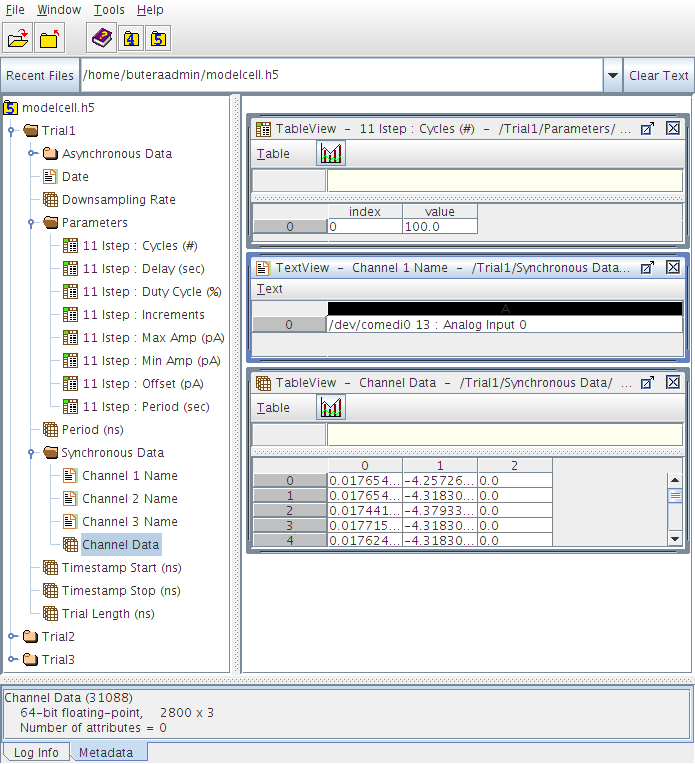
\includegraphics[width=6.5in]{axoclamptutorial5.png} 
\caption[HDF5]{RTXI uses a hierarchical HDF5 data structure organized into \emph{Trials}. Each \emph{Trial} contains the system settings and parameter values for that trial. This screenshot is taken using HDFView, a free software for browsing HDF5 files.} 
\label{fig:HDF5 structure}
\end{center}
\end{maxipage}
\end{figure}

\index{HDF5, MATLAB}There are various software available for working with HDF5 files. To simply browse the file structure, you can use the free HDFView application. HDFView provides some limited editing capabilities. For trials where only a single channel is saved, you can also preview a plot of the data. To extract the data for analysis and for complete editing capabilities, APIs are available for MATLAB, GNU Octave, Igor Pro, Mathematica, Python, Scilab, and other software. \marginlabel{MATLAB \& RTXI HDF5}For real-time streaming of multiple signals, an HDF5 data type is used in RTXI that does not map efficiently onto MATLAB native data types. While MATLAB can read this data using its low-level functions, this process can be very slow. To load RTXI HDF5 files quickly into MATLAB, you will first need to run a small utility function on your HDF5 file to convert the \emph{Synchronous Data} dataset to a different data type. This function is compiled when RTXI is compiled and is located in \texttt{/rtxi/hdf}. To convert your HDF5 file:\index{rtxi\_hdf\_matlabize}
\begin{example}
\$ rtxi\_hdf\_matlablize YOUR\_FILE.h5
\end{example}

To make this utility accessible from any directory on your system, make a symbolic link in \texttt{/usr/bin} to the location of this function in your RTXI source directory. If you installed RTXI from the Live CD, the source directory is \texttt{/home/rtxi}:
\begin{example}
\$ sudo ln -s RTXI\_SRC\_DIR/hdf/rtxi\_hdf\_matlabize \\ \hspace{1cm} /usr/bin/rtxi\_hdf\_matlabize
\end{example}

RTXI also includes a simple MATLAB GUI for quickly viewing the data within a single trial. The MATLAB code is available in \texttt{/rtxi/hdf/RTXIh5}. A sample m-file is provided with examples of how to extract data to the MATLAB workspace, how to use the GUI browser, and how to add new datasets to your file. It is also possible to embed binary formats, such as images, within a trial.

The GUI browser allows you to view the parameters, channels, and plots of the data within a single trial with the \texttt{rtxibrowse()} function. This generates a MATLAB figure window with the filename and trial number in the menu bar. To browse trials within the same HDF5 file, use the buttons in the lower left corner. The left panel lists the initial values for all the module parameters. If a parameter value has changed during the recording, this is denoted with an asterisk. The new values and their timestamps can be viewed by using the \texttt{getTrial()} function, which returns a MATLAB structure containing all the information within a trial. The GUI plots two channels from the same trial. Use the middle upper and and lower panels to select the data that is plotted in the right upper and lower panels. Double-clicking on a channel name in the middle panel will create a new figure window with that data plotted. This allows you to continue browsing through other trials in the main GUI window while keeping this additional plot available.

\begin{figure}[h!]
\begin{maxipage}
\begin{center}
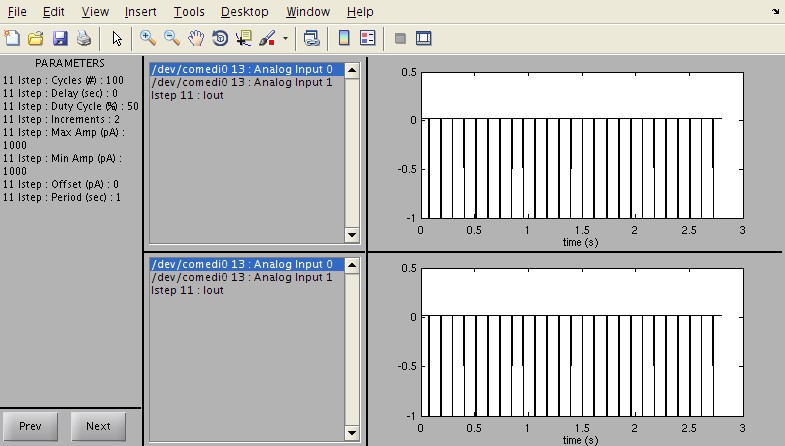
\includegraphics[width=6.5in]{axoclamptutorial6.png} 
\caption[RTXI HDF5 MATLAB GUI]{The MATLAB GUI browser allows you to view the parameters, channels, and plots of the data within a single trial.} 
\label{fig:HDF5 MATLAB}
\end{center}
\end{maxipage}
\end{figure}

%%%%%%%%%%%%%%%%%%%%%%%%%%%%%%%%%%%%%%%%%%%%%%%%%%%%%%%%%%%%

\chapter{RTXI Software Installation}
\index{installation}
There are two methods for installing RTXI on your computer:
\begin{enumerate}
\item Booting off an Ubuntu-based RTXI Live CD.
\item Compiling a real-time Linux operating system and RTXI from scratch.
\end{enumerate}

We suggest that users new to Linux start out with the Live CD. We have chosen Ubuntu since it is one of the most popular desktop distributions and has an extensive online support community. If you choose to compile the operating system yourself, you can choose any Linux distribution though there will be some minor differences in the installation steps. All Linux distributions are based on the same Linux ``kernel," but they differ in the utilities and libraries that are included by default. This leads to different desktop environments and applications.In general, you can expect to find a Linux application for just about anything you need to do. For some users, the manual compilation will result in better real-time performance. In particular, the 64-bit live CD is configured for a generic 64-bit processor and configuring the kernel for a specific processor family can result in lower latencies.

\attention
The current live CDs available on the RTXI website (http://www.rtxi.org) are configured to handle processors with either one or two cores. If your system has more cores, RTXI will not start off the live CD. You will know if this is the issue by checking your kernel log:
\bigskip
\begin{example}
\hrule\bigskip
\$ dmesg\\
.\\
.\\
$\left[\textrm{ 390.069252}\right] \textrm{RTAI}\left[\textrm{hal}\right]$: RTAI CONFIGURED WITH LESS THAN NUM ONLINE CPUS
\bigskip
\hrule\bigskip
\end{example}

To start Ubuntu with fewer cores enabled, press ``E" when you see the GRUB bootloader menu to edit the boot command. At the end of the line beginning with ``\texttt{boot}" and probably also containing the flags \texttt{quiet splash}, add the flag \texttt{maxcpus="2"} or whatever number of cores you want to use. to boot with this modification, use the keyboard shortcut CTRL-X. This modification is not permanent and you will need to do this step every time you restart the computer. Alternatively you can edit the GRUB menu to add this flag permanently.

\attention Note that Live CDs based on later Linux kernel version will support a wider variety of and more recent hardware.

%%%%%%%%%%%%%%%%%%%%%%%%%%%%%%%%%%%%%%%%%%%%%%%%%%%%

\section{Hardware Requirements}

\index{hardware requirements} \index{compatibility, hardware}
RTXI is designed to run on a standard personal desktop computer. The primary limitation is that the computer components must be supported by Linux and for this reason, the latest cutting-edge computing hardware, particularly advanced motherboards and graphics cards, is not recommended. The version the Linux kernel that may be used is also limited by the real-time support that is provided. For example, the RTAI project releases patches for the vanilla Linux kernel that are specific for different kernel versions. It is only possible to create a real-time kernel for supported kernel versions. \seealso{Chapter \ref{manualinstall}}
For more details, see the manual installation notes.

\index{real-time performance}Uniprocessor, multi-core processors, and multiple CPUs with and without hyperthreading are supported by Linux and RTXI. RTAI must be correctly configured for multiple cores to be used. More stable systems are typically realized with Intel processors rather than AMD processors. In rare cases, a particular CPU and motherboard combination is not supported. Certain advanced motherboards may contain features that are not compatible with RTAI. For example, some that use integrated graphics chips use hardware techniques to speed up computation that are also not compatible. An external video card is recommended and NVIDIA cards tend to have better Linux support than ATI/Radeon cards. This can be important since the greatest overhead in RTXI is related to data visualization in the oscilloscope. For newer graphics cards, you may need to manually install the Linux drivers, which are usually available on the manufacturer's website. Some systems may also include BIOS level or hardware interrupts that are not captured by RTAI or advanced power management features (sometimes these can be turned off by the user in the BIOS).

The real-time Linux kernel has extremely low latencies and little software overhead. RTXI is also designed so that the minimum number of dynamic modules can be loaded at any time. RTXI has been successfully run on computers with Pentium III processors up to 6-core Intel Xeon processors. While the processor speed allows RTXI to complete more computations within a single real-time cycle, the amount of RAM and the amount of video memory have a significant impact on the stability and speed of the system. Users should also consider high speed hard drives, large cache sizes, and high speed bus interfaces. If you are purchasing an off-the-shelf desktop computer system and plan to add a DAQ card, be sure that your power supply is powerful enough to handle the extra load. At least a 450W power supply is recommended.

\section{Data Acquisition Cards and COMEDI support}
\label{COMEDIsupport}
\index{COMEDI}

For closed loop experiments using RTXI, your computer must be equipped with an analog-to-digital converter (ADC) to acquire data and a digital-to-analog converter (DAC) to generate signals. Of course, external hardware such as an oscilloscope or function (waveform) generator can be used in conjunction with RTXI. A popular solution is to purchase a commercial multifunction data acquisition card that provides analog input and output, digital input and output, and counter/timer circuitry. DAQ cards using the USB interface are \attention \emph{not compatible} with RTXI since the USB drivers in Linux are not capable of hard real-time operation. Furthermore, the USB interface can only achieve a maximum sampling rate of approximately 1 kHz, which may be sufficient for some closed-loop real-time applications but not for \index{dynamic clamp}dynamic clamp. Many DAQ cards using the PCI, PCI express, or PXI interface are available from a variety of manufacturers. Your choice of DAQ card should depend on the number of analog and/or digital channels that you need, the amount of data resolution (eg. 12, 16-bit), the amount of sampling resolution (determined by the speed of the card), and whether you need simultaneous sampling (rather than sequential sampling) of multiple input channels. 

Most RTXI users use products developed by National Instruments. \attention A complete list of COMEDI supported DAQ cards is available at http://www.comedi.org. COMEDI also provides low-level drivers for cards using a 8255 chip, which provides three channels of 8 bit digital input or output, and for standard PC parallel ports. A list of currently supported NI cards and the corresponding COMEDI driver name is given in Table \ref{COMEDI NI}. A list of other COMEDI supported DAQ manufacturers is given in Table \ref{COMEDI DAQ}.\index{hardware requirements}

\vspace{1cm}
\begin{table}[htdp]
\caption{DAQ Manufacturers with COMEDI supported Hardware}
\label{COMEDI DAQ}
\begin{center}
\vspace{.5cm}
\begin{tabular}{ll}
ADLINK & http://www. adlinktech.com\\
Advantech & http://www.advantech.com\\
Amplicon & http://www.amplicon.com\\
Data Translation & http://www.datatranslation.com\\
Fastwel & http://www.fastwel.com\\
General Standards Corporation & http://www.generalstandards.com\\
ICP & http://www.icpdas-usa.com\\
Intelligent Instrumentation & http://www.instrument.com\\
Keithley Instruments & http://www.keithley.com\\
Measurement Computing & http://www.mccdaq.com\\
National Instruments & http://www.ni.com/dataacquisition\\
\end{tabular}
\end{center}
\end{table}
\vspace{1cm}

\begin{fullpage}
\begin{table}
\caption{COMEDI supported National Instruments DAQ cards}
\label{COMEDI NI}
\begin{center}
\vspace{.5cm}
\begin{tabular}{lcclc}
 \textbf{Device} & \textbf{Driver} & & \textbf{Device} & \textbf{Driver}\\
AT-MIO-16E-1 & ni\_atmio & & PCI-MIO-16XE-50 & ni\_pcimio\\ 
AT-MIO-16E-2 & ni\_atmio & & PCI-MIO-16XE-10 & ni\_pcimio\\ 
AT-MIO-16E-10 & ni\_atmio & & PCI-MIO-16E-1 & ni\_pcimio\\ 
AT-MIO-16DE-10 & ni\_atmio & & PCI-MIO-16E-4 & ni\_pcimio\\ 
AT-MIO-64E-3 & ni\_atmio & & PCI-6014 & ni\_pcimio\\ 
AT-MIO-16XE-50 & ni\_atmio & & PCI-6030E & ni\_pcimio\\ 
AT-MIO-16XE-10 & ni\_atmio & & PCI-6040E & ni\_pcimio\\ 
AT-AI-16XE-10 & ni\_atmio &  & PCI-6031E & ni\_pcimio\\ 

& & & PCI-6033E & ni\_pcimio\\ 
PCIe-6251 & ni\_pcimio &  & PCI-6071E & ni\_pcimio\\ 
PCIe-6259 & ni\_pcimio &  & PCI-6023E & ni\_pcimio\\ 

& & & PCI-6024E & ni\_pcimio\\ 
PXI-6030E & ni\_pcimio &  & PCI-6025E & ni\_pcimio\\ 
PXI-6040E & ni\_pcimio &  & PCI-6034E & ni\_pcimio\\ 
PXI-6025E & ni\_pcimio &  & PCI-6035E & ni\_pcimio\\ 
PXI-6281 & ni\_pcimio &  & PCI-6036E & ni\_pcimio\\ 
PXI-6711 & ni\_pcimio &  & PCI-6052E & ni\_pcimio\\ 
PXI-6713 & ni\_pcimio &  & PCI-6070E & ni\_pcimio\\ 
PXI-6071E & ni\_pcimio &  & PCI-6110 & ni\_pcimio\\ 
PXI-6070E & ni\_pcimio &  & PCI-6111 & ni\_pcimio\\ 
PXI-6052E & ni\_pcimio &  & PCI-6143 & ni\_pcimio\\ 
PXI-6733 & ni\_pcimio &  & PCI-6220 & ni\_pcimio\\ 
PXI-6143 & ni\_pcimio &  & PCI-6221 & ni\_pcimio\\ 
& & & PCI-6224 & ni\_pcimio\\ 
& & & PCI-6225 & ni\_pcimio\\ 
& & & PCI-6229 & ni\_pcimio\\ 
& & & PCI-6250 & ni\_pcimio\\ 
& & & PCI-6251 & ni\_pcimio\\ 
& & & PCI-6254 & ni\_pcimio\\ 
& & & PCI-6259 & ni\_pcimio\\ 
& & & PCI-6280 & ni\_pcimio\\ 
& & & PCI-6281 & ni\_pcimio\\ 
& & & PCI-6284 & ni\_pcimio\\ 
& & & PCI-6289 & ni\_pcimio\\ 
& & & PCI-6711 & ni\_pcimio\\ 
& & & PCI-6713 & ni\_pcimio\\ 
& & & PCI-6731 & ni\_pcimio\\ 
& & & PCI-6733 & ni\_pcimio\\ 
\end{tabular}
\end{center}
\end{table}
\end{fullpage}

\label{more DAQ cards}\attention RTXI has no built-in software limitations on the number of DAQ cards but is configured for only one card by default. If you want to use additional cards, you will need to edit the configuration file. Here is the relevant excerpt of \texttt{/etc/rtxi.conf}:\index{DAQ, multiple cards}\index{RTXI, configuration}
\begin{example}
\bigskip\hrule\smallskip
<OBJECT component="plugin" library="comedi\_driver.so" id="2">\\
<PARAM name="0">/dev/comedi0</PARAM>\\
<PARAM name="Num Devices">1</PARAM>\\
<OBJECT id="13" name="0" />\\
</OBJECT>
\bigskip\hrule\bigskip
\end{example}

Edit the lines to add another COMEDI device and change the number of devices:
\begin{example}
\bigskip\hrule\smallskip
<PARAM name="0">/dev/comedi0</PARAM>\\
<PARAM name="1">/dev/comedi1</PARAM>\\
<PARAM name="Num Devices">2</PARAM>
\bigskip\hrule\bigskip
\end{example}

You will need to exit and restart RTXI for the new configuration to take effect. Settings files that you have already created should still work when you change \texttt{rtxi.conf} but you may not have access to both DAQ cards in the System Control Panel, the Oscilloscope, and the Connector. You will have to rebuild those settings files or edit them as above using your choice of text editor.

RTXI automatically detects the manufacturer and board names of available DAQ cards and the number and type of input and output channels. The first DAQ card installed in your system is assigned the Linux device name: \texttt{/dev/comedi0}. Additional DAQ cards are assigned device names \texttt{/dev/comedi1} and so on. You can check that your DAQ card has been correctly detected and see the corresponding device name by clicking \textbf{Help}$\rightarrow$\textbf{About COMEDI} from the RTXI menu bar.

\index{DAQ, calibration} \index{calibration}
\index{COMEDI, calibration}\label{comedi calibration}
To calibrate your DAQ card, use the comedi\_calibrate utility as follows for each COMEDI device:
\begin{example}
\$ sudo comedi\_calibrate --reset --dump --calibrate --results --verbose /dev/comedi0
\end{example}

If you are using a National Instruments M-Series card, you will need to use the \texttt{comedi\_soft\_calibrate} utility instead.

%%%%%%%%%%%%%%%%%%%%%%%%%%%%%%%%%%%%%%%%%%%%%%%%%%%%
\section{Live CD Installation}
\label{liveCD}\index{RTXI, Live CD} \index{Live CD} \index{installation, Live CD}

The Live CD provides a complete real-time Linux operating system with RTXI without installing anything on your computer. This live environment allows you to mount your existing hard drive and you can conduct experiments and collect data. Note that the real-time performance will be slower compared with an actually installed system. Running the live environment from a USB flash drive is faster than from an actual CD. The Live CD is available in both 32 and 64-bit versions. Currently, the 32-bit version is available for Ubuntu 8.04 Hardy Heron and Ubuntu 9.10 Karmic Koala. The 64-bit version is available for Ubuntu 9.10 Karmic Koala. For older computers, the Ubuntu 8.04 version may work better. If the live environment successfully loads and RTXI is functioning, then the installation of the system to your hardware will typically go smoothly. The live CD should be the first test for any new RTXI setup. The following screenshots are taken from Ubuntu 9.10.

To decrease the size of the Live CD, many common desktop applications, such as OpenOffice, were removed. These can be reinstalled using the Applications menu in Ubuntu.

\bigskip\bigskip
\hrule
You do not need a DAQ card installed to test the live CD or for RTXI to run.
\bigskip
\hrule
\bigskip

\begin{enumerate}
\item Download the live CD that corresponds to your processor architecture. if you are not sure, try the 32-bit live CD. A 32-bit CD based on Ubuntu 8.04 Hardy Heron may be more successful on older computers.

\item Burn the *.iso image to a CD/DVD or load it onto a USB flash drive. In both cases, you should make sure that your BIOS is set to boot from an available CD/USB before the internal hard drive. To burn the image to a CD, you will need to have this option in your CD burning software. You cannot simply copy the *.iso image to the disk. To load the image onto a USB flash drive, we commend using Ubuntu's USB Disk Creator. On Ubuntu 9.10, you can find this application in the menu bar under System$\rightarrow$Administration. If it is not there, you may install it by:
\begin{example}
\$ sudo apt-get install usb-creator
\end{example}

Point the application to the *.iso image you just downloaded and to a USB flash drive. The drive should be partitioned as FAT32, but if it is incorrectly formatted, the application will you an option to reformat it. It also gives you an option to enable ``persistence" on the USB drive, allowing you to save files and change settings in the live user sessions that will be there the next time you boot off the live USB. You cannot change the size of the persistence file after you have created the live USB, so make it as large as you might need. The USB will work on Windows and Linux computers but not Mac computers.
\begin{figure}[h]
\begin{center}
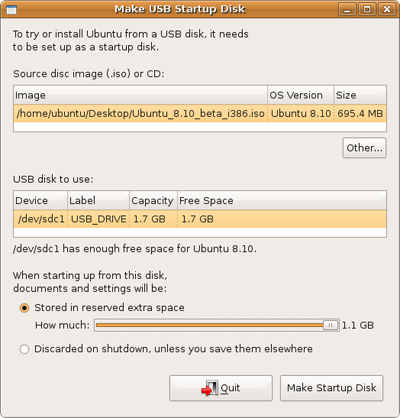
\includegraphics{Usb-creator.png} 
\caption[Ubuntu USB Disk Creator]{The USB Disk Creator allows you to create a bootable Ubuntu USB flash drive from an *.iso image file.} 
\end{center}
\end{figure}

\newpage
\item Boot your computer off the CD or USB. You may need to modify your BIOS settings to give the CD/USB device boot priority over your hard drive. In some cases, Ubuntu will correctly load but will drop you to a shell prompt rather than the GUI. This is usually due to video drivers that were not bundled directly into the kernel or were not able to be loaded. If you see a shell prompt, try starting the GUI by typing:
\begin{example}
\# startx
\end{example}

\item If you have at least 512MB of RAM, you may want to select ``Try Ubuntu without any change to your computer." This will the operating system and give a live user session. You will be able to connect to the Internet and use any Ubuntu applications. You can find the real-time benchmark tests in the RTXI folder under the Applications menu in the menu bar. You may also choose to go straight to the installer by double-clicking the ``Install" icon on the desktop.

\item Answer all the setup questions. If you are in the U.S., the default options will probably already be what you want.

\item By default, the installer will give you the option to install Ubuntu side by side with whatever operating system is currently on your computer. If you want to dual-boot Ubuntu with another operating system, choose the very last option to set up your partitions manually. Click Forward. Below is an example of a computer with two hard drives, each of which has a single partition defined. \texttt{sda} refers to the first hard drive connected to your motherboard (in this case the SATA0 slot) and \texttt{sdb} is the second hard drive. If you have IDE rather than SATA hard drives, you should see \texttt{hda} drive designations. \texttt{sda1} is the first and only partition on the first hard drive. Since it contains a Windows installation, we see that it�s formatted as NTFS. The second hard drive has about 35GB of free space in which to create new partitions for Linux.
\begin{figure}[h]
\begin{center}
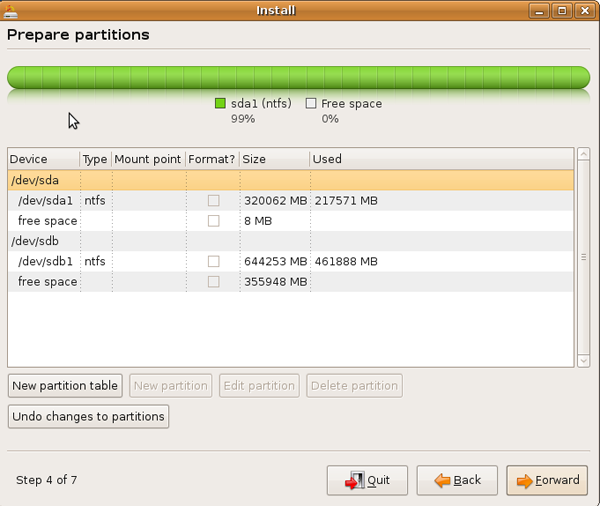
\includegraphics[width=4.5in]{livecd1.png} 
\caption[Ubuntu Installation: Preparing your partitions]{The Ubuntu installer allows you to reconfigure your partitions. This configuration shows a single Windows partition (\texttt{/dev/sdb1}) in NTFS file format that uses the entire second hard drive (\texttt{/dev/sdb}).} 
\end{center}
\end{figure}

\item If you already have a Windows partition on your hard drive, you probably don�t have any free space for Linux. To resize a partition, click on it (eg. \texttt{/dev/sdb1}) and then click ``Edit Partition." You will get a pop-up window with a colored bar representing the partition. Use your mouse to drag the right edge of the colored bar so that the partition is smaller, leaving you with unallocated free space at the end. Hit ``OK" and you should see that on \texttt{/dev/sdb} you have a \texttt{/dev/sdab} partition and more free space.

\item Linux uses a special \texttt{swap} partition that is used to augment the RAM and increase the total amount of virtual memory that is available to running applications. If you have 3-4GB of RAM, you probably don�t need any more, but you can make a 1-2GB swap space just in case. If you only have 1-2GB of RAM, you should add 2GB of swap space. Click on the free space in your partition table and click ``New Partition." The default size of a new partition is the rest of the free space on the hard drive so decrease it to the desired size of your swap partition and select the type as ``swap."

\item For the actual Linux OS, make another new partition in the remaining free space. This one should be a ``Primary" partition and set the mount point to be a single forward-slash ``/", which indicates that it�s the root location. Ubuntu 9.10 defaults to the new ext4 filesystem format but it occasionally has problems so you might want to set the type to ext3. You may also want to leave some extra room for a data partition that is read/write-able in both Windows and Linux. This partition should be formatted as NTFS or FAT32. Note that FAT32 can only handle file sizes up to 4GB. You can have up to 4 primary partitions. If you need more, you need to create an �extended� partition under which you can create as many ``logical" partitions as you like.
\begin{figure}[h]
\begin{center}
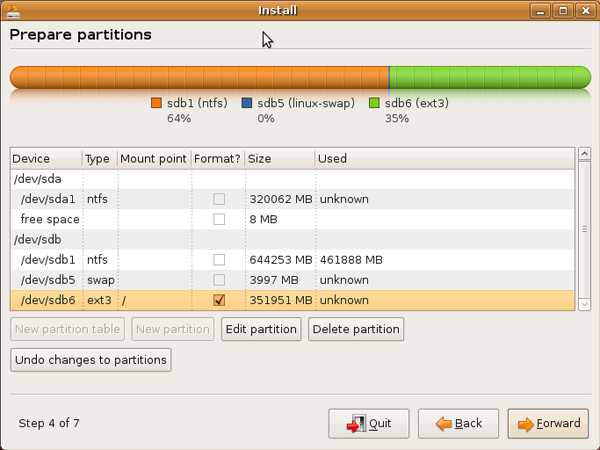
\includegraphics[width=4.5in]{livecd2.png} 
\caption[Ubuntu Installation: Dual booting Window and Linux]{This configuration shows a hard drive (\texttt{/dev/sdb}) partitioned to dual boot Windows and Linux. The Windows NTFS formatted partition remains and was simply resized. There are additional Linux swap and Linux ext3 formatted partitions as well. The ext3 partition is set to the root \texttt{/} mount point and has been selected to be formatted. The NTFS partition is NOT going to be formatted so no data will be lost.} \end{center}
\end{figure}

\item Your new Linux partition should have a flag indicating that the hard drive space will be formatted. If you are dual-booting, make sure your Windows (NTFS) partition is NOT set to be formatted if you want to keep your data. When you�re all done setting up your partitions, click ``Forward." You can always restart the hard drive partitioner in Linux to resize your partitions. If you decide you need more room in Linux, you can make the Windows partition a little smaller, creating free space between the Windows and other partitions. Then, move over the swap partition and increase the size of the Linux partitioner. If you want multiple Linux installations on the same hard drive, they will all use the same swap space, so you only ever need one swap partition.

\item Ubuntu 9.10 will ask you if you want to import user settings from any other available OS. Then it will start installing the OS, including a new bootloader called GRUB. When you reboot your computer, you will get a menu that asks whether you want Windows or Linux. If you re-install Windows, it will overwrite GRUB and you will no longer be able to boot into Linux even if its partition still exists there. In that case, you need to reinstall GRUB using a Live CD.

\item You can start RTXI from the Applications menu or from the terminal:
\begin{example}
\$ rtxi
\end{example}

\end{enumerate}

%%%%%%%%%%%%%%%%%%%%%%%%%%%%%%%%%%%%%%%%%%%%%%%%%%%%
\section{Manual Installation}
\label{manualinstall} \index{installation, manual}

The following instructions are provided for the Ubuntu Linux distribution. Other Linux distributions are compatible with RTXI and can be used following similar steps for compiling a real-time kernel, installing RTAI, and installing RTXI and its package dependencies. Differences you can expect during the procedure include different commands for compiling a new kernel, different commands for retrieving packages from the distribution's repository, different package names, and different ways of loading RTAI kernel modules at start up. RTXI  has been successfully installed on SUSE and Fedora Linux. Unless otherwise noted, the following package names are consistent with the repositories for Ubuntu versions 8.10/9.04/9.10. The required version numbers for Linux, RTAI and other packages may vary for different versions of Ubuntu and other Linux distributions.
\index{compatibility, software}
\begin{table}[htdp]
\caption{Successfully tested RTXI installations (not exhaustive). The first column gives the Ubuntu version that was installed using an official Live CD as well as the vanilla Linux kernel version that was used for building an RTAI-based real-time kernel.}
\begin{center}
\vspace{.5cm}
\begin{tabular}{lccc}
\textbf{Linux kernel)} & \textbf{RTAI} & \textbf{COMEDI} & \textbf{HDF5}\\
Ubuntu 8.04 (2.6.29.4) & 3.8.1 & 0.7.76 & 1.8.4\\
Ubuntu 9.10 (2.6.29.4) & 3.8.1 & 0.7.76 &1.8.4/1.8.6\\
Ubuntu 9.10 (26.31.1) & 3.8.1 & 0.7.76 & 1.8.4-1.8.7\\
Ubuntu 10.04 (26.32.11) & 3.8.1 & Git & 1.8.7
\end{tabular}
\end{center}
\label{default}
\end{table}%


All lines beginning with ``\texttt{\$}" are commands to execute in the terminal. Use the TAB key to allow the shell to autocomplete directory and filenames for you.

\begin{enumerate}
\item Install a clean version of Ubuntu (probably using their Live CD). The RTXI Live CD installation steps can guide you through this process. Be sure to choose the desktop (not the server) version and the appropriate 32 or 64-bit version. It will ask you to create an initial user.
\item Login as the user you created. We will use the \texttt{sudo} command to get superuser administrative privileges. Do not install RTAI when logged in as root. It will not work.
\item Get the required packages for Ubuntu.  These commands will look for the packages in the Ubuntu repository, identify any dependencies they have, and tell you how much additional space you need to install everything. Just hit \texttt{ENTER} to accept all the default options and install.
\begin{example}
\$ sudo apt-get update\footnote{``\texttt{sudo}'' gives you superuser adminstrative privileges. Enter the root password at the prompt. This command updates the list of packages that are available in the Ubuntu repository.}\\
\$ sudo apt-get upgrade\footnote{This installs any updates for all packages you currently have installed.}\\
\$ sudo apt-get install cvs subversion build-essential\\
\$ sudo apt-get install kernel-package linux-source\\
\$ sudo apt-get install libncurses5-dev libtool automake\\
\$ sudo apt-get install bison flex qt3-dev-tools\\
\$ sudo apt-get install libboost-dev libgsl0-dev\\
\$ sudo apt-get install libboost-program-options-dev\footnote{For Ubuntu 10.04, the correct package name is \texttt{libboost-program-options1.40-dev}.}
\end{example}

\item Determine which version of the Linux kernel you have and select a corresponding RTAI release.
\begin{example}
\$ cat /proc/version
\end{example}
This tells you your current kernel version (Linux version 2.6.\#\#.\#) as well as your gcc compiler version. Grab a copy of RTAI and check the available kernel patches. Versions older than 3.7 are not compatible with gcc 4.3.3. To get the latest CVS (development) version that will be compatible with more recent kernel versions:
\begin{example}
\$ cd /opt\footnote{``\texttt{cd}" is the command to change directories. The \texttt{/opt} directory is usually reserved for software and add-on packages that are not part of the default installation.}\\
\$ sudo cvs -d:pserver:anonymous@cvs.gna.org:/cvs/rtai co magma\\
\$ sudo ln -s magma rtai\footnote{This creates a symbolic link so that \texttt{rtai} points to the \texttt{magma} folder. This saves you some typing. Type \begin{example}\$ ls -al\end{example} in the terminal to see how this works. This command lists all the files and directories in your current directory with their user permissions and date of modification.} 
\end{example}

To get a stable release version (replacing the version number with the one you want):
\begin{maxipage}
\begin{example}
\$ cd /opt\\
\$ sudo wget --no-check-certificate https://www.rtai.org/RTAI/rtai-3.8.1.tar.bz2\footnote{This is a compressed format. The next line will extract the folder.}\\
\$ sudo tar xjvf rtai-3.8.1.tar.bz2\\
\$ sudo ln -s rtai-3.8.1 rtai
\end{example}
\end{maxipage}

Navigate to the patches directory for your particular hardware e.g. \texttt{/opt/rtai/base/arch/x86/patches}.\footnote{There are other folders for other processor architectures. The x86\_64 label has been deprecated and the x86 folder contains the necessary patches for both 32 and 64-bit Intel and AMD desktop processors.} List all the available patches in that folder:
\begin{example}
\$ ls
\end{example}

Find the highest Linux kernel version that matches yours. For example, you might have kernel version 2.6.28-generic and see RTAI patches:
\begin{example}
hal-linux-2.6.28.2-x86-2.2.05.patch\\
hal-linux-2.6.28.7-x86-2.2.06.patch\\
hal-linux-2.6.28.9-x86-2.2.07.patch
\end{example}
You should download the vanilla (the official �clean�) kernel 2.6.28.9.

\item Get the kernel that corresponds to your kernel version number.
\begin{maxipage}
\begin{example}
\$ cd /usr/src\\
\$ sudo wget http://www.kernel.org/pub/linux/kernel/v2.6/linux-2.6.29.4.tar.bz2\\
\$ sudo tar xjvf linux-2.6.29.4.tar.bz2\\
\$ sudo ln -s linux-2.6.29.4 linux
\end{example}
\end{maxipage}

\item Patch the kernel with the RTAI patch you identified in step 4.
\begin{maxipage}
\begin{example}
\$ cd /usr/src/linux\\
\$ sudo patch -p1 < /opt/rtai/base/arch/x86/patches/hal-linux-2.6.28.9-x86-2.2.07.patch
\end{example}
\end{maxipage}
You should see messages about files being patched. If you see messages about ``hunks" failing, then the patch was not compatible with that version of the Linux kernel. The RTAI patch does not usually correctly patch kernel source code on which a patch has previously been applied. To try again, delete the folder with the extracted kernel source code and re-extract a fresh directory:

\begin{example}
\$ cd /usr/src\\
\$ sudo rm -r linux-2.6.29.4\footnote{``\texttt{rm}" is the command to delete a file. To delete a directory, you must add the ``\texttt{-r}" flag. Since \texttt{/usr/src} is an important protected system directory, you need administrator privileges to perform this operation.} \\
\$ sudo tar xjvf linux-2.6.29.4.tar.bz2\\
\end{example}

\item Configure the kernel. We will take your existing configuration as a foundation (since we know it is a working configuration) and then make some modifications. 
\begin{example}
\$ cd /usr/src/linux\\
\$ sudo cp /boot/config-\textasciigrave uname -r\textasciigrave.config\footnote{This command copies the kernel configuration file from your \texttt{/boot} directory to \texttt{/usr/src/linux/.config}. The ` in the first command is not a regular single quote, but rather the kind on the $\sim$ (tilde) key.} \\
\$ sudo make oldconfig
\end{example}

You will probably be prompted about many configuration options. Accept the default option by pressing return for each one. Using this method, you will have a large kernel that has support for many devices compiled directly into the kernel or as loadable modules. To make a smaller kernel, disable some features you know you don't need. An obvious one would be tablet or touchscreen input support. To make the kernel significantly smaller, you can disable kernel debugging. The following command will create a menu for configuring the kernel for real-time. If you do not see ``Adeos," ``Interrupt pipeline," or ``IPIPE" options, the RTAI patch did not work. 
\begin{example}
\$ sudo make menuconfig
\end{example}

This menu uses the keyboard for navigation. To get a GUI menu that allows you to use the mouse and search for configuration options, use:
\begin{example}
\$ sudo make xconfig
\end{example}

Below is a sample kernel configuration. Not all of the options that are listed here may appear in your menu. You should configure those options that you do see as shown. 

\index{COMEDI}Kernel versions 2.6.30 and later have an experimental in-tree COMEDI implementation in the driver "staging" area. RTAI support for the in-tree "staging" version is still in development, so for current RTAI releases the Git version of COMEDI should be used. To avoid module inconsistencies later, you may want to opt out of compiling the COMEDI kernel staging drivers.

\begin{fullpage}\index{kernel configuration}
\begin{maxipage}
\begin{example}
General setup\\
\hspace{.5cm}Set "Local version - append to kernel release" to "-adeos"  $\left[\textrm{or whatever you want}\right]$\\

Enable loadable module support\\
\hspace{.5cm}$ \left[\ast\right]$ Module unloading\\  
\hspace{.5cm}$\left[ \hspace{.2cm}\right]$ Module versioning support\\

Processor type and features\\
\hspace{.5cm}$\left[\ast\right]$ Symmetric multi-processing support\\
\hspace{.5cm}$\left[\hspace{.2cm}\right]$ Support sparse irq numbering\footnote{Disable this feature if you get the following error when compiling. Happily, this error occurs very early in the process: \begin{example}include/linux/ipipe.h:76:2 error: \#error �CONFIG\_NR\_CPUS is too large, please lower it\end{example}
} \\
\hspace{.5cm}Processor family to �Pentium-4/Celeron/Pentium-4 M/older Xeon�  $\left[\textrm{whatever you have}\right]$\\

\hspace{.5cm}Preemption Model ---> Preemptible Kernel (Low-Latency Desktop)\footnote{Ubuntu 8.04/8.10/9.10 can be compiled successfully with RTAI using the Low-Latency Desktop option . Ubuntu 10.04 may need the Voluntary Preemption option instead. Some users report that the Grub2 bootloader sometimes does not work with the low-latency option. This can be circumvented by downgrading back to Grub1. The low-latency option does results in better real-time performance for RTXI.}\\
\hspace{.5cm}$\left[\ast\right]$ Interrupt pipeline\\
\hspace{.5cm}$\left[\ast\right]$ Local APIC support on uniprocessors\\
\hspace{1cm}$\left[\ast\right]$ IO-APIC support on uniprocessors\\

Power management and ACPI options\\
\hspace{.5cm}$\left[\ast\right]$ Power Management support\\
\hspace{.5cm}$\left[\hspace{.2cm}\right]$ Suspend to RAM and standby\\
\hspace{.5cm}$\left[\hspace{.2cm}\right]$ Hibernation\\
\hspace{.5cm}$\left[\ast\right]$ ACPI (Advanced Configuration and Power Interface Support)\\
\hspace{1cm}$\left[\hspace{.2cm}\right]$ AC Adapter\\
\hspace{1cm}$\left[\hspace{.2cm}\right]$ Battery\\
\hspace{1cm}$\left[\hspace{.2cm}\right]$ Button\\
\hspace{1cm}$\left[\ast\right]$ Fan\\
\hspace{1cm}$\left[\ast\right]$ Dock\\
\hspace{1cm}$\left[\ast\right]$ Processor\\
\hspace{1cm}$\left[\ast\right]$ Thermal Zone\\
\hspace{1cm}$\left[\hspace{.2cm}\right]$ Smart Battery System\\
\hspace{.5cm}CPU Frequency scaling\\
\hspace{1cm}$\left[\hspace{.2cm}\right]$ CPU Frequency scaling\\

Device Drivers \\
\hspace{.5cm}$\left[\ast\right]$ Staging drivers\\
\hspace{1cm}$\left[\hspace{.2cm}\right]$ Data acquisition support (comedi)\\


Kernel hacking \\
\hspace{.5cm}$\left[\hspace{.2cm}\right]$ KGDB: kernel debugging with remote gdb\\
\end{example}
\end{maxipage}
\end{fullpage}

\item Compile the custom kernel and install it. This will take a long time. You will get a series of .deb packages that can be copied and installed onto other computers so that you don�t have to compile the entire kernel again. If you do this, the computers need to have similar specifications, e.g. the same kind of processor, the same original Linux kernel version. If these do not match, the real-time performance will not be optimized or the kernel may even fail to boot. Alternatively, if you have multiple computers with the same hardware configuration, you may copy the configuration file you created and recompile the .deb packages.
\begin{example}
\$ sudo make-kpkg clean\footnote{\texttt{make-kpkg} is a script which automates and replaces the sequence : \texttt{make dep}, \texttt{make clean}, \texttt{make bzImage}, \texttt{make modules}. These commands are typical kernel compilation steps for other popular Linux distributions. Always run \texttt{make-kpkg clean} before compiling a new kernel.} \\
\$ sudo make-kpkg --initrd kernel\_image kernel\_headers kernel\_source
\end{example}

If your folder permissions are incorrect, you may get the following error when you try to compile:
\begin{example}
dpkg-deb: control directory has bad permissions 2755 (must be >=0755 and <=0755)
\end{example}

You will have to ``clean" and recompile after executing the following to fix the permissions:
\begin{example}
\$ chmod �R a-s /usr/src
\end{example}

\item Install the custom real-time kernel.
\begin{maxipage}
\begin{example}
\$ cd /usr/src\\
\$ sudo dpkg -i linux-headers-2.6.29.4-adeos\_2.6.29.4-adeos-10.00.Custom\_i386.deb\\
\$ sudo dpkg -i linux-image-2.6.29.4-adeos\_2.6.29.4-adeos-10.00.Custom\_i386.deb\footnote{The Linux bootloader is called Grub and after installing a new kernel, the file \texttt{/boot/grub/menu.lst} should be automatically updated so that you can choose your new kernel when booting. View this file to manually check this. You will need sudo access to manually edit it. Ubuntu versions 9.10 and later use Grub2, which will automatically detect all the operating systems in every partition that it finds when it updates Grub. Grub2 replaces \texttt{menu.lst} with \texttt{grub.cfg}.} 
\end{example}
\end{maxipage}

\item Boot into your new real-time kernel!\footnote{If you have a newer system with an NVIDIA graphics card, for example,the correct driver may not be compiled into the kernel. You will get a terminal interface (no GUI because it couldn�t start an X server) and some messages that might say something like it found the monitor but couldn�t set any profiles or that it could not find a screen. Reboot into your default kernel and download the NVIDIA driver. Reboot to the real-time kernel, navigate to the location where you downloaded the driver and follow the NVIDIA instructions to manually install it. }
\begin{example}
\$ sudo reboot
\end{example}

\item Verify how many processor cores are recognized by the kernel. If you have a multi-core processor you will see some output for each CPU.
\begin{example}
\$ cat /proc/cpuinfo
\end{example}

\item Configure and install RTAI without COMEDI support for now. Make sure you select the correct number of CPUs or none of the RTAI modules will load. \index{RTAI, configuration}
\begin{example}
\$ cd /opt/rtai\\
\$ sudo make menuconfig
\end{example}

\begin{maxipage}
\begin{example}
General\\
\hspace{.5cm}Installation ---> /usr/realtime\\
\hspace{.5cm}Kernel source ---> /usr/src/linux\\
Machine\\
\hspace{.5cm}(\#) Number of CPUs (SMP-only)\\
Other Features\\
\hspace{.5cm}$\left[\ast\right]$ User space interrupts\footnote{This option should be enabled for Ubuntu versions 10.04 and later. It may also be needed for certain multicore processors. This is likely the case if RTXI fails to load. \texttt{CTRL-C} will abort the loading of RTXI and give you a backtrace of the error. If you see an error referring to \texttt{sem\_wait}, enable the RTAI user space interrupts and try again.}\\
Add-ons\\
\hspace{.5cm}$\left[\hspace{.2cm}\right]$ Real Time COMEDI support in user space
\end{example}
\end{maxipage}

You may get an error that the Linux directory must be specified, in which case you will have to configure RTAI from the terminal:
\begin{maxipage}
\begin{example}
\$ sudo ./configure --with-linux-dir=/usr/src/linux --enable-testsuite --disable-rtailab\\
\$ sudo make clean \\
\$ sudo make\\
\$ sudo make install
\end{example}
\end{maxipage}

If you get the following error during compilation, reconfigure RTAI without leds-based debugging support.
\begin{maxipage}
\begin{example}
../../../base/include/asm/rtai\_leds.h:24:20: error: asm/io.h: No such file or directory\\ 
\vspace{.2cm}
\$ sudo ./configure --with-linux-dir=/usr/src/linux --enable-testsuite --disable-rtailab\        --disable-leds\\
\$ sudo make clean \\
\$ sudo make\\
\$ sudo make install
\end{example}
\end{maxipage}

\item Tell your system where to find the real-time scripts. In each open shell of the terminal:
\begin{example}
\$ export PATH=/usr/realtime/bin:\$PATH
\end{example}

\item Test the real-time performance of your system. The operating system splits memory into kernel space, reserved for running the kernel and some device drivers, and user space, which is where user applications run. In \texttt{/usr/realtime/testsuite} there are two folders, \texttt{/kern} and \texttt{/user}, containing benchmark tests for kernel space and user space. In the latency folder run:
\begin{example}
\$ sudo ./run
\end{example}

\seealso{Chapter \ref{Latency Test}\\RTAI Latency Test}
If the latency test fails, you will probably get a ``kernel panic" that freezes your entire system. This indicates that your kernel is configured incorrectly and you are not running a hard real-time operating system. This is the most important benchmark test and the first test that you should run. You want to see zeroes in the very last column labeled ``overruns." To stop the test, press \texttt{CTRL-C}. More information about RTAI real-time benchmark tests are available in Chapter \ref{RTAI benchmarks}.

\item Get the COMEDI drivers. A snapshot of COMEDI 0.7.76 is hosted in the RTXI repository and has been used with Ubuntu 8.04/8.10/9.10. 
\begin{maxipage}
\begin{example}
\$ cd /opt\\
\$ svn co https://rtxi.svn.sourceforge.net/svnroot/rtxi/trunk/comedi comedi\\
\$ svn co https://rtxi.svn.sourceforge.net/svnroot/rtxi/trunk/comedilib comedilib\\
\$ svn co https://rtxi.svn.sourceforge.net/svnroot/rtxi/trunk/comedi\_calibrate comedi\_calibrate\\
\end{example}
\end{maxipage}

The recommended way to install COMEDI and Comedilib is to compile from the current Git source, as the released versions are quite old (in particular, comedi-0.7.76 only supports kernels up to 2.6.24). Kernel versions 2.6.30 onwards have an experimental in-tree COMEDI implementation in the driver "staging" area. This support should improve with later kernel versions. Note that RTAI support for the in-tree "staging" version is still in development, so for current RTAI releases the Git version of COMEDI should be used.

\begin{maxipage}
\begin{example}
\$ sudo apt-get install git-core\\
\$ sudo git clone git://comedi.org/git/comedi/comedi.git\\
\$ sudo git clone git://comedi.org/git/comedi/comedilib.git\\
\$ sudo git clone git://comedi.org/git/comedi/comedi\_calibrate.git
\end{example}
\end{maxipage}

\item Configure, compile, and install COMEDILIB.
\begin{example}
\$ cd /opt/comedilib\\
\$ sudo sh autogen.sh\\
\$ sudo ./configure \\
\$ sudo make\\
\$ sudo make install
\end{example}

\item Configure, compile, and install COMEDI\_CALIBRATE.
\begin{example}
\$ cd /opt/comedi\_calibrate\\
\$ sudo autoreconf -i \\
\$ sudo ./configure\\
\$ sudo make\\
\$ sudo make install
\end{example}

Under Ubuntu 9.10, configure may fail and give a \texttt{libboost-program-options} error.  In \texttt{/usr/lib}, list all the libboost libraries:
\begin{example}
\$ ls | grep libboost
\end{example}

You may have \texttt{libboost\_program\_options-mt} rather than\\ \texttt{libboost-program\_options}. You will need to change any references to this library to the correct library name. In the file \texttt{/opt/comedi\_calibrate/configure.ac}, find the line:
\begin{maxipage}
\begin{example}
$AC\_CHECK\_LIB(\left[boost\_program\_options\right],\left[main\right],,$\\
\hspace{1cm}$AC\_MSG\_ERROR(\left[\textrm{Failed to find }libboost\_program\_options.\right]))$
\end{example}
\end{maxipage}

Change \texttt{boost\_program\_options} in the first argument to\\ \texttt{boost\_program\_options-mt}. You also need to edit\\ \texttt{/comedi/comedi\_soft\_calibrate/Makefile.am}. In the line beginning with \texttt{comedi\_soft\_calibrate\_LDADD}, change \texttt{�lboost\_program\_options} to \texttt{�lboost\_program\_options-mt}. Repeat all commands in step 17 to configure COMEDI\_CALIBRATE.

\item Configure, compile, and install COMEDI.
\begin{example}
\$ cd /opt/comedi\\
\$ sudo sh autogen.sh\\
\$ sudo ./configure \\
\$ sudo make\\
\$ sudo make install\\
\$ sudo mkdir -p /usr/local/include/linux\\
\$ sudo cp include/linux/comedi.h include/linux/comedilib.h /usr/local/include/linux\footnote{These last two steps are not necessary when compiling COMEDI Git against Ubuntu 10.04.}
\end{example}

To calibrate your card, use \texttt{comedi\_calibrate}, or \texttt{comedi\_soft\_calibrate} if you have a M-series NI card.
\begin{example}
\$ sudo comedi\_calibrate /dev/comedi0\\
\end{example}

\item Configure and install RTAI with COMEDI support.\index{RTAI, configuration}
\begin{example}
\$ cd /opt/rtai\\
\$ sudo make menuconfig
\end{example}

\begin{maxipage}
\begin{example}
General\\
\hspace{.5cm}Installation ---> /usr/realtime\\
\hspace{.5cm}Kernel source ---> /usr/src/linux\\
Machine\\
\hspace{.5cm}(\#) Number of CPUs (SMP-only)\\
Other Features\\
\hspace{.5cm}$\left[\ast\right]$ User space interrupts\footnote{This option should be enabled for Ubuntu versions 10.04 and later. It may also be needed for certain multicore processors. This is likely the case if RTXI fails to load. \texttt{CTRL-C} will abort the loading of RTXI and give you a backtrace of the error. If you see an error referring to \texttt{sem\_wait}, enable the RTAI user space interrupts and try again.}\\
Add-ons\\
\hspace{.5cm}$\left[\ast\right]$ Real Time COMEDI support in user space\\
\hspace{.5cm}COMEDI installation directory ---> /opt/comedi
\end{example}
\end{maxipage}

Or configure RTAI from the terminal:
\begin{maxipage}
\begin{example}
\$ sudo ./configure --with-linux-dir=/usr/src/linux --enable-testsuite --disable-rtailab\ 
--disable-leds --enable-comedi-lxrt --with-comedi=/opt/comedi\\

\$ sudo make\\
\$ sudo make install
\end{example}
\end{maxipage}

If you made a mistake configuring RTAI, you must uninstall COMEDI and COMEDILIB before reinstalling RTAI. COMEDI must be compiled with real-time support so it has to be built after RTAI. To uninstall, go to the \texttt{comedi} and \texttt{comedlib} directories and:
\begin{example}
\$ sudo make uninstall\\
\$ sudo make clean
\end{example}

\item To use RTAI, you must have the necessary RTAI and COMEDI kernel modules loaded. Create these scripts to load all the modules we need for RTXI. You may use any text editor you like. The following command will open the nano text editor and create the file \texttt{rtaiinsmod} in \texttt{/usr/realtime/bin}, the installation directory for other RTAI scripts :\footnote{*DRIVER* is the COMEDI driver you will be using, e.g. \texttt{ni\_pcimio}. If you have an older NI E-Series card, you may need to use the \texttt{ni\_atmio} driver. These cards may be detected as Plug and Play (PnP) devices, which you can check by typing \begin{example}\$ dmesg\end{example} and looking for them. This driver has 2.6 kernel support and should automatically probe for a supported board. If your board is not recognized, download the \texttt{isapnptools} package from http://www.roestock.demon.co.uk/isapnptools/.} 

\begin{example}
\$ sudo nano /usr/realtime/bin/rtaiinsmod
\end{example}

Copy the following text into your new file and replace *DRIVER* with the correct COMEDI driver for your DAQ card:

\begin{maxipage}
\begin{example}
\# Inserts RTAI and COMEDI modules in kernel and configures the drivers.\\
\vspace{.5cm}
insmod /usr/realtime/modules/rtai\_hal.ko\\
insmod /usr/realtime/modules/rtai\_lxrt.ko\\
insmod /usr/realtime/modules/rtai\_sem.ko\\
insmod /usr/realtime/modules/rtai\_shm.ko\\
modprobe kcomedilib\\
insmod /usr/realtime/modules/rtai\_comedi.ko\\
\vspace{.5cm}
\# Hardware dependent lines below. \\
modprobe *DRIVER*
\end{example}
\end{maxipage}
The keyboard shortcut \texttt{CTRL-O} will allow you to save the file. Use \texttt{CTRL-X} to exit. Now create a script that you can use to quickly remove RTAI and COMEDI modules from the kernel:
\begin{example}
\$ sudo nano /usr/realtime/bin/rtairmmod
\end{example}
\begin{maxipage}
\begin{example}
\# Removes RTAI and COMEDI modules from kernel.\\
\vspace{.5cm}
modprobe -r *DRIVER*\\
\vspace{.5cm}
rmmod rtai\_comedi\\
modprobe -r kcomedilib\\
rmmod rtai\_shm\\
rmmod rtai\_sem\\
rmmod rtai\_lxrt\\
rmmod rtai\_hal\\
\end{example}
\end{maxipage}
Make these scripts executable\footnote{\texttt{chmod} changes the user permissions for a file or directory. Type \texttt{ls -al} to see how this works. The first field is a list of 10 permission flags. The first contains a 'd' if it is a directory and is '-', otherwise. The next set of three fields are the read, write, and execute permissions for the User or Owner of the file. The next three are the permissions for the Group, and the last three are the permissions for any other users. A '-' in any position means that the flag is not set. \texttt{r}, \texttt{w}, and \texttt{x} means that the file is readable, writeable, or executable, respectively. A permission of \texttt{-rw-rw----} means that you and anyone else in your group have read and write access to the file. The command below adds the executable flag to the scripts you created. To remove a flag, you would use the minus sign instead of the addition sign.}:
\begin{example}
\$ sudo chmod +x /usr/realtime/bin/rtaiinsmod\\
\$ sudo chmod +x /usr/realtime/bin/rtairmmod
\end{example}

\item Now let�s execute your script automagically when you boot the kernel. Open \texttt{/etc/rc.local} for editing. Add a line to the end before the ``\texttt{exit 0}":

\begin{maxipage}
\begin{example}
\#!/bin/sh -e\\
\#\\
\# rc.local\\
\#\\
\# This script is executed at the end of each multiuser runlevel.\\
\#\\
\# By default this script does nothing.\\
\vspace{.5cm}
/usr/realtime/bin/rtaiinsmod\\
exit 0\\
\end{example}
\end{maxipage}

Reboot and check that all the modules listed in your script have been loaded:
\begin{example}
\$ lsmod | grep rtai\footnote{\texttt{lsmod} lists all the currently loaded kernel modules. The vertical bar indicates that you would like to execute a command on the output of \texttt{lsmod}. The \texttt{grep} command searches text for ``rtai" and has the effect of filtering the output of \texttt{lsmod}.}
\end{example}

You can also check the kernel log to see that RTAI is registered, that the scheduler and timer are set up, the version of COMEDI that is loaded, and the IDs of any available DAQ cards:
\begin{example}
\$ dmesg
\end{example}

\item Install the HDF5 libraries in the correct location. Previous versions of the HDF5 source code is located at\\ http://www.hdfgroup.org/ftp/HDF5/prev-releases/.
\begin{maxipage}
\begin{example}
\$ cd /opt\\
\$ sudo wget http://www.hdfgroup.org/ftp/HDF5/current/src/hdf5-1.8.7.tar.gz\\
\$ sudo tar xvf hdf5-1.8.7.tar.gz\\
\$ cd hdf5-1.8.7\\
\$ sudo ./configure --prefix=/usr \\
\$ sudo make\\
\$ sudo make install
\end{example}
\end{maxipage}

You may also want to get the graphical HDFView application that will let you explore your file (http://www.hdfgroup.org/HDF5/).

\item Grab RTXI from our SourceForge subversion repository. Put it in your user's home folder.\footnote{To update RTXI, repeat the \texttt{svn} command. You may want to make a backup copy of the entire \texttt{/rtxi} folder first so that you can restore the old version if the new one doesn�t work.}\index{RTXI, source code repository}
\begin{maxipage}
\begin{example}
Currently, the "trunk" branch of the RTXI repository is version 1.2. It contains snapshots of the COMEDI, COMEDILIB, and COMEDI\_CALIBRATE source code that were used for the Ubuntu 9.10 Live CD and for manual installations of RTXI for that kernel version.\\
\vspace{.5cm}
\$ cd \$HOME\\
\$ svn co https://rtxi.svn.sourceforge.net/svnroot/rtxi/trunk rtxi\\
\vspace{.5cm}
RTXI v1.3 is still undergoing testing and is available as a branch.\\
\vspace{.5cm}
\$ cd \$HOME\\
\$ svn co https://rtxi.svn.sourceforge.net/svnroot/rtxi/branches/1.3 rtxi
\end{example}
\end{maxipage}

\item Configure, compile, and install RTXI.
\begin{example}
\$ cd rtxi\\
\$ sh autogen.sh\\
\$ ./configure
\end{example}

If the QT library is installed somewhere that RTXI doesn�t look, you will probably get an error about not having a working QT installation. It tests this by trying to compile a small QT application. Configure RTXI with the correct location of QT, e.g.:
\begin{example}
\$ ./configure �-with-Qt-dir=/usr/qt\\
\$ ./configure �-with-Qt-dir=/usr/lib/qt3
\end{example}

Now:
\begin{example}
\$ make\\
\$ sudo make install
\end{example}

In Ubuntu 9.10, or any distribution with autoconf$>$2.63, autogen.sh may produce a configure script that fails with an \texttt{fi} syntax error when checking for a QT installation. This is caused by an empty if -then-else-fi structure produced by the \texttt{BNV\_HAVE\_QT} macro in \texttt{autogen.sh}. In the \texttt{/rtxi/m4} folder, edit \texttt{bnv\_have\_qt.m4}. Around line 510, you should see a line with this comment:

\begin{example}
\bigskip
\hrule
\bigskip
\# Leave bnv\_qt\_lib\_dir undefined
\bigskip
\hrule
\bigskip
\end{example}

Add a line before this line that is a colon �:� all by itself:
\begin{example}
\bigskip
\hrule
\bigskip
:\\
\# Leave bnv\_qt\_lib\_dir undefined
\bigskip
\hrule
\end{example}

The colon is a �no-operation� statement for the shell and works around the syntax error. Instead of the file \texttt{bnv\_have\_qt.m4}, you may have the file \texttt{ax\_have\_qt.m4}. They are essentially the same file and the same instructions apply.

\item Start RTXI from the terminal. If you did not reboot to test your scripts for automatically loading the RTAI and COMEDI modules, you will have to manually insert them first:
\begin{example}
\$ cd /usr/realtime/bin\\
\$ sudo ./rtaiinsmod\\
\$ rtxi
\end{example}
In whatever terminal window you start RTXI from, you will see any error messages, debugging messages you write in your code, etc. If you do not have a DAQ card installed, you will see a warning about COMEDI. You may still use RTXI without a DAQ card, including compiling and testing custom user modules.  If you see an error about not being able to load \texttt{/etc/rtxi.conf}, copy it there:
\begin{example}
\$ sudo cp \$HOME/rtxi/rtxi.conf /etc\\
\$ rtxi
\end{example}

\item If you need DYNAMO, you will need to compile the DYNAMO translation utility.
\begin{example}
\$ sudo apt-get install mlton\\
\$ cd /rtxi/dynamo\\
\$ mllex dl.lex\\
\$ mlyacc dl.grm\\
\$ mlton dynamo.mlb\\
\$ sudo cp dynamo /usr/bin
\end{example}

\end{enumerate}
 \label{install DYNAMO}
%%%%%%%%%%%%%%%%%%%%%%%%%%%%%%%%%%%%%%%%%%%%%%%%%%%%%%%%%%%%
\newpage
\section{RTXI Configuration Options}
\index{RTXI, configuration}
RTXI can be manually configured with other options. For example, you may want to run RTXI using the Xenomai real-time interface rather than RTAI or in non-real-time mode using the POSIX interface for debugging purposes. You may also direct RTXI to libraries/packages in non-standard locations. The full configuration options are below:

\begin{maxipage}
\begin{example}
Usage: ./configure [OPTION]... [VAR=VALUE]...To assign environment variables (e.g., CC, CFLAGS...), specify them as VAR=VALUE.  See below for descriptions of some of the useful variables. Defaults for the options are specified in brackets.

Configuration:\\ \vspace{.4cm}
\begin{tabular}{ll}
-h, --help              &     display this help and exit\\
--help=short           &    display options specific to this package\\
--help=recursive    &   display the short help of all the included packages\\
-V, --version           &    display version information and exit\\
-q, --quiet, --silent   &  do not print `checking...' messages\\
--cache-file=FILE   &  cache test results in FILE [disabled]\\
-C, --config-cache    &    alias for `--cache-file=config.cache'\\
-n, --no-create       &    do not create output files\\
--srcdir=DIR     &     find the sources in DIR [configure dir or `..']\\
\end{tabular}

Installation directories:\\ \vspace{.4cm}
\begin{tabular}{ll}
--prefix=PREFIX       &    install architecture-independent files in PREFIX \\
& [/usr/local]\\
--exec-prefix=EPREFIX   &  install architecture-dependent files in EPREFIX [PREFIX]
\end{tabular}

By default, `make install' will install all the files in
`/usr/local/bin', `/usr/local/lib' etc.  You can specify
an installation prefix other than `/usr/local' using `--prefix',
for instance `--prefix=\$HOME'.

For better control, use the options below.\\ \vspace{.4cm}

Fine tuning of the installation directories:\\ \vspace{.4cm}
\begin{tabular}{ll}
--bindir=DIR         &     user executables [EPREFIX/bin]\\
--sbindir=DIR       &      system admin executables [EPREFIX/sbin]\\
--libexecdir=DIR    &      program executables [EPREFIX/libexec]\\
--sysconfdir=DIR      &    read-only single-machine data [PREFIX/etc]\\
--sharedstatedir=DIR    &  modifiable architecture-independent data [PREFIX/com]\\
--localstatedir=DIR    &   modifiable single-machine data [PREFIX/var]\\
--libdir=DIR     &         object code libraries [EPREFIX/lib]\\
--includedir=DIR     &     C header files [PREFIX/include]\\
--oldincludedir=DIR  &     C header files for non-gcc [/usr/include]\\
--datarootdir=DIR    &     read-only arch.-independent data root [PREFIX/share]\\
--datadir=DIR       &      read-only architecture-independent data [DATAROOTDIR]\\
\end{tabular}

\end{example}
\end{maxipage}

\begin{maxipage}
\begin{example}
\begin{tabular}{ll}
--infodir=DIR        &     info documentation [DATAROOTDIR/info]\\
--localedir=DIR   &        locale-dependent data [DATAROOTDIR/locale]\\
--mandir=DIR     &         man documentation [DATAROOTDIR/man]\\
--docdir=DIR      &        documentation root [DATAROOTDIR/doc/rtxi]\\
--htmldir=DIR     &        html documentation [DOCDIR]\\
--dvidir=DIR       &       dvi documentation [DOCDIR]\\
--pdfdir=DIR      &        pdf documentation [DOCDIR]\\
--psdir=DIR      &         ps documentation [DOCDIR]
\end{tabular}



Program names:\\ \vspace{.4cm}
\begin{tabular}{ll}
--program-prefix=PREFIX    &          prepend PREFIX to installed program names\\
--program-suffix=SUFFIX      &        append SUFFIX to installed program names\\
--program-transform-name=PROGRAM   &  run sed PROGRAM on installed program names
\end{tabular}


X features:\\ \vspace{.4cm}
\begin{tabular}{ll}
--x-includes=DIR   &   X include files are in DIR\\
--x-libraries=DIR  &   X library files are in DIR
\end{tabular}

System types:\\ \vspace{.4cm}
\begin{tabular}{ll}
--build=BUILD    &   configure for building on BUILD [guessed]\\
--host=HOST     &    cross-compile to build programs to run on HOST [BUILD]
\end{tabular}

Optional Features:\\ \vspace{.4cm}
\begin{tabular}{ll}
--disable-option-checking &   ignore unrecognized --enable/--with options\\
--disable-FEATURE     &  do not include FEATURE (same as --enable-FEATURE=no)\\
--enable-FEATURE[=ARG]  &  include FEATURE [ARG=yes]\\
--enable-shared[=PKGS]   & build shared libraries [default=yes]\\
--enable-static[=PKGS]  &  build static libraries [default=yes]\\
--enable-fast-install[=PKGS]  & optimize for fast installation [default=yes]\\
--disable-dependency-tracking  &  speeds up one-time build\\
--enable-dependency-tracking   &  do not reject slow dependency extractors\\
--disable-libtool-lock  &  avoid locking (might break parallel builds)\\
--enable-xenomai      &   build the Xenomai interface\\
--enable-posix      &     build the POSIX non-RT interface\\
--enable-debug       &    turn on debugging\\
--enable-comedi    &      build the comedi driver\\
--enable-ni        &      build the ni driver
\end{tabular}

Optional Packages:\\ \vspace{.4cm}
\begin{tabular}{ll}
--with-PACKAGE[=ARG]    &  use PACKAGE [ARG=yes]\\
--without-PACKAGE      &   do not use PACKAGE (same as --with-PACKAGE=no)\\
--with-cppunit-prefix=PFX   &  Prefix where CppUnit is installed (optional)\\
--with-cppunit-exec-prefix=PFX   & Exec prefix where CppUnit is installed (optional)\\
--with-pic       &         try to use only PIC/non-PIC objects [default=use both]\\
--with-gnu-ld       &      assume the C compiler uses GNU ld [default=no]\\
--with-x            &      use the X Window System\\
\end{tabular}
\end{example}
\end{maxipage}

\begin{maxipage}
\begin{example}
\begin{tabular}{ll}

--with-Qt-dir=DIR      &   DIR is equal to \$QTDIR if you have followed the \\
& installation instructions of Trolltech. Header files \\
& are in DIR/include, binary utilities are in DIR/bin. \\
& The library is in DIR/lib, unless --with-Qt-lib-dir \\
& is also set.\\
--with-Qt-include-dir=DIR  & Qt header files are in DIR\\
--with-Qt-bin-dir=DIR  &   Qt utilities such as moc and uic are in DIR\\
--with-Qt-lib-dir=DIR   &  The Qt library is in DIR\\
--with-Qt-lib=LIB      &   Use -lLIB to link with the Qt library\\
--with-rtai-config=FILE  & location of the rtai-config program
\end{tabular}

Some influential environment variables:\\ \vspace{.4cm}
\begin{tabular}{ll}
CC      &      C compiler command\\
CFLAGS    &    C compiler flags\\
LDFLAGS   &    linker flags, e.g. -L<lib dir> if you have libraries in a nonstandard\\
&  directory <lib dir>\\
LIBS   &       libraries to pass to the linker, e.g. -l<library>\\
CPPFLAGS  &    C/C++/Objective C preprocessor flags, e.g. -I<include dir> if you have\\
& headers in a nonstandard directory <include dir>\\
CPP       &    C preprocessor\\
CXX       &    C++ compiler command\\
CXXFLAGS   &   C++ compiler flags\\
CXXCPP    &    C++ preprocessor\\
XMKMF     &    Path to xmkmf, Makefile generator for X Window System
\end{tabular}

Use these variables to override the choices made by `configure' or to help
it to find libraries and programs with nonstandard names/locations.

\end{example}
\end{maxipage}


%%%%%%%%%%%%%%%%%%%%%%%%%%%%%%%%%%%%%%%%%%%%%%%%%%%%%%%%%%%%

\chapter{Writing Custom User Modules}
\label{custommodules}
\index{modules, custom}

\section{Using the \texttt{DefaultGUIModel} Class}
\label{defaultGUImodules}
\index{DefaultGUIModel}
\index{modules, DefaultGUIModel}

User modules are actually custom C\texttt{++} classes. The easiest way to create a module is to use a base class named \texttt{DefaultGUIModel}. \texttt{DefaultGUIModel} constructs a simple graphical user interface that allow users to interact with parameters and activate real-time code. These modules also inherit methods for hard real-time execution and event handling, the ability to generate and accept signals, and the ability to have metadata automatically captured by the Data Recorder to HDF5 data files. The following sections describe the \texttt{Neuron} module, which provides a Hodgkin-Huxley model neuron that generates a membrane voltage signal and accepts an optional external current input. The GUI consists of a column of textboxes and associated labels to display the module's parameters and internal state variables. Each instantiation of a user module is given a unique instance ID that appears in the left corner of the window's title bar. Parameters are editable variables and their textboxes are shown in black. The internal state variables of a module are traditionally considered intermediate computed values that should not be edited manually by the user. States are shown in gray. 
\begin{figure}[h!] 
\begin{center}
\label{NeuronGUI}
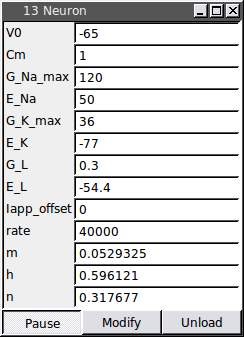
\includegraphics[width=2.1in]{hhneuron.png} 
\caption[Neuron GUI]{The \texttt{Neuron} module is a Hodgkin-Huxley model neuron described by conductance-based differential equations. This GUI provides an interface by which a user can modify parameters, such as the conductance of the ion channels, on-the-fly and start and stop real-time execution of the module} 
\end{center}
\end{figure}

\subsection{Creating your own module class}

The quickest way to create a new user module is to duplicate an existing module directory and rename the files and the class. This involves renaming the class header (*.h) file, the class implementation (*.cpp) file, editing the Makefile and editing any instances of the old class name within each of these files. The latter include the class name, scope names, the constructor, and the deconstructor. A template user module is available in \texttt{/rtxi/doc/my\_plugin}.

\subsection{Edit the Makefile}
The Makefile instructs the compiler how to build your module and link it to RTXI. In RTXI v1.2 and later, the Makefile allows modules to be compiled outside the core RTXI source tree. A sample Makefile (compatible with RTXI v1.2 and later) is provided below:
\begin{maxipage}\index{Makefile}
\begin{example}
PLUGIN\_NAME = my\_plugin  \\
\vspace{.5cm}
HEADERS = my\_plugin.h  \\
\vspace{.5cm}
SOURCES = my\_plugin.cpp $\backslash$ \\
\hspace{2cm}included\_class.h $\backslash$ \\
\hspace{2cm}Included\_class.cpp\\
\vspace{.5cm}
LIBS = -lgsl\\
\vspace{.5cm}
\#\#\# Do not edit below this line \#\#\# \\
include \$\$(shell rtxi\_plugin\_config --pkgdata-dir)/Makefile.plugin\_compile
\end{example}
\end{maxipage}

The \texttt{PLUGIN\_NAME} is the name that will be given the shared object library (*.so) file when it is compiled. All modules should be given unique names since the compilation process will automatically overwrite the library when installed to \texttt{/usr/local/lib/rtxi}. The \texttt{HEADERS} and \texttt{SOURCES} must be edited to reflect the new source file names. For simple modules based on a single class, there will be a single header file and a single source file. You may base your module on additional custom classes whose sources must then be included here as well. The \texttt{LIBS} flag is used for any additional library flags. Here, \texttt{-lgsl} links this module against the GNU Scientific Library.

\subsection{Define model parameters, inputs, and outputs}

\texttt{DefaultGUIModel} uses a special workspace variable \texttt{vars[]} to define quantities in the module, generate a GUI, and implement certain features such as module inputs and outputs and changing parameter values on-the-fly. The declaration of these types follows a simple syntax. Every \texttt{DefaultGUIModel} \attention module must have a workspace variable called \texttt{variable\_t} as shown below. 

\begin{maxipage}
\begin{example}
static DefaultGUIModel::variable\_t vars$\left[\right]$ =\\
\{\\
\hspace{.5cm}\{"Iapp", "A", DefaultGUIModel::INPUT,\},\\
\hspace{.5cm}\{"Vm", "V", DefaultGUIModel::OUTPUT,\},\\
\hspace{.5cm}\{"V0", "mV", DefaultGUIModel::PARAMETER|DefaultGUIModel::DOUBLE,\},\\
\hspace{.5cm}\{"Cm", "uF/cm$^{\wedge}$2", DefaultGUIModel::PARAMETER|DefaultGUIModel::DOUBLE,\},\\
\hspace{.5cm}\{"G\_Na\_max", "mS/cm$^{\wedge}$2", DefaultGUIModel::PARAMETER|DefaultGUIModel::DOUBLE,\},\\
\hspace{.5cm}\{"E\_Na", "mV", DefaultGUIModel::PARAMETER|DefaultGUIModel::DOUBLE,\},\\
\hspace{.5cm}\{"G\_K\_max", "mS/cm$^{\wedge}$2", DefaultGUIModel::PARAMETER|DefaultGUIModel::DOUBLE,\},\\
\hspace{.5cm}\{"E\_K", "mV", DefaultGUIModel::PARAMETER|DefaultGUIModel::DOUBLE,\},\\
\hspace{.5cm}\{"G\_L", "mS/cm$^{\wedge}$2", DefaultGUIModel::PARAMETER|DefaultGUIModel::DOUBLE,\},\\
\hspace{.5cm}\{"E\_L", "mV", DefaultGUIModel::PARAMETER|DefaultGUIModel::DOUBLE,\},\\
\hspace{.5cm}\{"rate", "Hz",  DefaultGUIModel::PARAMETER|DefaultGUIModel::UINTEGER,\},\\
\hspace{.5cm}\{"m" "Sodium Activation", DefaultGUIModel::STATE,\},\\
\hspace{.5cm}\{"h", "Sodium Inactivation", DefaultGUIModel::STATE,\},\\
\hspace{.5cm}\{"n", "Potassium Activation", DefaultGUIModel::STATE,\},\\
\};
\end{example}
\end{maxipage}

Each element in \texttt{vars[]} defines an \texttt{INPUT}, \texttt{OUTPUT}, \texttt{PARAMETER}, \texttt{STATE} variable, or \texttt{COMMENT} for the module. The first argument for each element is the label for the textbox in the GUI. This does not have to be the same as the variable name you use in the code to actually store the parameter value. The second argument is displayed as a Tooltip when you use your mouse to hover the cursor over that entry in the GUI. Enter any descriptive information here about the variable, such as an expanded form of your text label or the correct units of measurement. The third argument defines the variable as an input, output, etc. Notice that for parameters, you can also specify whether it is a double or integer numeric type. 

Declaring an \texttt{INPUT} creates a slot for your module to acquire data from the DAQ card or from another module. Declaring an \texttt{OUTPUT} creates a signal that is emitted from your module that can be send to your DAQ card or any other module. These inputs and outputs will be accessible when you open the Connector module or the Data Recorder module. In the example code below, there is only one input, Iapp, and its value is accessed as the variable \texttt{input(0)}. The values of additional inputs would be accessed as \texttt{input(1)}, \texttt{input(2)}, and so on. The same rule applies for outputs eg. the value of Vm is accessed as \texttt{output(0)}. These references may be used in other member functions for your custom module.

\texttt{STATE} variables and \texttt{PARAMETER}s are numeric datatypes. State variables are internal model variables that cannot be modified by the user through the GUI. Their values may be constant or they may change over time. It is common to use a \texttt{STATE} to track the values of intermediate or computed quantities. These state variables can also be saved by the Data Recorder. A \texttt{PARAMETER} will accept user input through the GUI and can be modified on the fly during real-time execution. State variables and parameters appear in the GUI in the order that they are declared. However, state variables are not editable and are displayed in gray. You can simply monitor the values of the state variables as they change. In the example code, this mechanism is used to monitor the ion channel's activation variables, which are dependent on membrane voltage and integrated in real-time. A \texttt{COMMENT} is similar to a \texttt{PARAMETER}, but is used to store text strings such as information about the experiment that you would like to log. These are saved to the Data Recorder just like parameters, but should not be modified in real-time during model execution.

\attention If your parameter name contains a forward slash ``/", its values will not be automatically saved by the Data Recorder. This is a limitation of the HDF5 file format, which uses a directory-like syntax for specifying the data structure.

\subsection{Initialize the model}

The next section is the model constructor. If you changed the class name, this would read ``\texttt{YOURMODEL::YOURMODEL}". You can set the text that will appear in the title bar of your module window using the first argument of the constructor method. \attention The next required line is a call to the \texttt{createGUI()} function which actually generates the GUI shown in Figure \ref{NeuronGUI}.\footnote{\texttt{createGUI()} is only required in RTXI v1.3 and later.}  In this section, you should initialize all the variables and parameter values and make sure that the GUI reflects the actual values that are being used. In this example, much of this code is performed by the \seealso{Chapter \ref{DefaultGUIModel update}\\\texttt{update()}} \texttt{update()} function under the \texttt{INIT} flag. In other modules downloadable from our website, you will find a separate \texttt{initParameters()} function that handles all variable initializations. 

It is convenient to perform unit conversions when calling these functions so that the GUI accepts input in more user-friendly units. Finally, you should call \texttt{refresh()} to update the GUI to reflect your changes. The GUI textboxes will be initialized to the current values of the variables and \texttt{STATE} variables will be updated periodically during model execution. 
\begin{maxipage}
\begin{example}
Neuron::Neuron(void) : DefaultGUIModel("Neuron", ::vars, ::num\_vars) $\{$\\
\hspace{.5cm}createGUI(vars, num\_vars); // creates the GUI\\ 
\hspace{.5cm}V = V0;\\
\hspace{.5cm}m = m\_inf(V0);\\
\hspace{.5cm}h = h\_inf(V0);\\
\hspace{.5cm}n = n\_inf(V0);\\
\hspace{.5cm}period = RT::System::getInstance()->getPeriod() * 1e-6; // convert ns to ms\\
\hspace{.5cm}update(INIT); // calls the update() function with the INIT flag\\
\hspace{.5cm}refresh(); // refreshes the GUI to reflect parameter values stored in variables\\
$\}$
\end{example}
\end{maxipage}

Notice the method for retrieving the real-time period (sampling rate) of the system:
\begin{example}\index{RT::System::getInstance()-$>$getPeriod()}
RT::System::getInstance()->getPeriod();
\end{example}

This returns the period in nanoseconds. 

\subsection{The execute() loop}
\label{DefaultGUIModel execute}
The \texttt{execute()} function will run to completion on every time step. The computations performed here must complete within the real-time period that you have set in the \seealso{Chapter \ref{system control panel} \\System Control Panel}System Control panel to maintain system stability. The efficiency of your code here will affect the performance of your system. You should use private variables defined in the class header rather than creating variables inside the function on every time step. If you absolutely must create a variable inside \texttt{execute()}, use a static call so that the same memory block is used each time. \attention You should be wary of using \texttt{do-while} and \texttt{for} structures if you are uncertain how long these loops will take to complete. Within the execute function, you must also be careful to bound the output signal and perform your own error checking to maintain the stability of the closed-loop. Notice that at the end, we have set \texttt{output(0)} to update the membrane voltage signal emitted by this module. RTXI's signals-and-slots architecture allows you to \attention connect any signal to any slot. There is no error checking that the connection is valid, eg. that quantities with matching units of measurement are connected.

\bigskip\hrule
\begin{example}
void Neuron::execute(void) $\{$\\
\hspace{.5cm}for (int i = 0; i < steps; ++i)\\
\hspace{1cm}solve(period / steps, y); // integrate equations\\
\hspace{.5cm}output(0) = V * 1e-3; // convert to mV\\
$\}$\\
\end{example}
\bigskip
\hrule

\subsection{The update() function}
\label{DefaultGUIModel update}

The \texttt{update{}} function is provided with several flags to help you organize your code and handle events in your module. The flags provided with the \texttt{DefaultGUIModel} class are:
\begin{itemize}
\item \texttt{INIT}: non-event related but useful for placing code to initialize the model
\item \texttt{MODIFY}: called when the "Modify" button is pressed
\item \texttt{PAUSE}: called when the model is paused
\item \texttt{UNPAUSE}: called when the model is unpaused
\label{pause flag}\item \texttt{PERIOD}: called when the real-time period of the system is changed
\end{itemize}


Under the \texttt{INIT} flag, you should initialize any additional variables or GUI settings that were not already addressed in the constructor. To assign a variable to be updated as a \texttt{STATE} variable in the GUI, use:
\begin{example}\index{setState()}
setState("YOUR\_GUI\_LABEL", YOUR\_VARIABLE);
\end{example}

\attention \texttt{YOUR\_GUI\_LABEL} must exactly match the label that you set in \texttt{variable\_t vars$\left[\right]$} above. Similarly, you initialize the GUI for a \texttt{PARAMETER} with:
\begin{example}\index{setParameter()}
setParameter("YOUR\_GUI\_LABEL", YOUR\_VARIABLE);
\end{example}

It is often the case that you may want to display units in the GUI with more convenient physiological units of measurement, eg. mV instead of V. In that case, you can call the function as follows:
\begin{example}\index{setParameter()}
setParameter("E\_Na", E\_Na*1000); // convert to mV\\
\end{example}

Under the \texttt{MODIFY} flag, you should grab all the values in the GUI textboxes and update the values of the parameters as follows:
\begin{example}
YOUR\_VARIABLE = getParameter("YOUR\_GUI\_LABEL").toDouble();
\end{example}

If you do any unit conversions with \texttt{setParameter()}, make sure you do the inverse with \texttt{getParameter()}. You may also want to add code to the \texttt{PAUSE} flag to set the output of your module to zero, e.g. the amplitude of an injected current. \attention In some cases, you will want to reset certain internal variables when you stop or start the model eg. a counter that keeps track of your model execution time. Under the \texttt{PERIOD} flag, you will always want to update your model with the new real-time period. 

\begin{maxipage}
\begin{example}
void Neuron::update(DefaultGUIModel::update\_flags\_t flag) $\{$\\
\hspace{.5cm}switch (flag) $\{$\\
\hspace{1cm}case INIT:\\
\hspace{1.5cm}setState("m", m);\\
\hspace{1.5cm}setState("h", h);\\
\hspace{1.5cm}setState("n", n);\\
\hspace{1.5cm}setParameter("V0", V0);\\
\hspace{1.5cm}setParameter("Cm", Cm);\\
\hspace{1.5cm}setParameter("G\_Na\_max", G\_Na\_max);\\
\hspace{1.5cm}setParameter("E\_Na", E\_Na);\\
\hspace{1.5cm}setParameter("G\_K\_max", G\_K\_max);\\
\hspace{1.5cm}setParameter("E\_K", E\_K);\\
\hspace{1.5cm}setParameter("G\_L", G\_L);\\
\hspace{1.5cm}setParameter("E\_L", E\_L);\\
\hspace{1.5cm}setParameter("Iapp\_offset", Iapp\_offset);\\
\hspace{1.5cm}setParameter("rate", rate);\\
\hspace{1.5cm}break;\\
\hspace{1cm}case MODIFY:\\
\hspace{1.5cm}V0 = getParameter("V0").toDouble();\\
\hspace{1.5cm}Cm = getParameter("Cm").toDouble();\\
\hspace{1.5cm}G\_Na\_max = getParameter("G\_Na\_max").toDouble();\\
\hspace{1.5cm}E\_Na = getParameter("E\_Na").toDouble();\\
\hspace{1.5cm}G\_K\_max = getParameter("G\_K\_max").toDouble();\\
\hspace{1.5cm}E\_K = getParameter("E\_K").toDouble();\\
\hspace{1.5cm}G\_L = getParameter("G\_L").toDouble();\\
\hspace{1.5cm}E\_L = getParameter("E\_L").toDouble();\\
\hspace{1.5cm}Iapp\_offset = getParameter("Iapp\_offset").toDouble();\\
\hspace{1.5cm}rate = getParameter("rate").toDouble();\\
\hspace{1.5cm}steps = static\_cast (ceil(period * rate / 1000.0));\\
\hspace{1.5cm}V = V0;\\
\hspace{1.5cm}m = m\_inf(V0);\\
\hspace{1.5cm}h = h\_inf(V0);\\
\hspace{1.5cm}n = n\_inf(V0);\\
\hspace{1.5cm}break;\\
\hspace{1cm}case PAUSE:\\
\hspace{1.5cm}break;\\
\hspace{1cm}case UNPAUSE:\\
\hspace{1.5cm}break;\\
\hspace{1cm}case PERIOD:\\
\hspace{1.5cm}period = RT::System::getInstance()->getPeriod() * 1e-6; // ms\\
\hspace{1.5cm}steps = static\_cast (ceil(period * rate / 1000.0));\\
\hspace{1.5cm}break;\\
\hspace{1cm}default:\\
\hspace{1.5cm}break;\\
\hspace{.5cm}$\}$\\
$\}$
\end{example}
\end{maxipage}

%%%%%%%%%%%%%%%%%%%%%%%%%%%%%%%%%%%%%%%%%%%%%%%%%%%

\section{DYNAMO Modules}
\label{dynamomodules}
\index{DYNAMO}
\index{modules, DYNAMO}
A complete manual for the DYNAMO class is given in Appendix \ref{dynamo appendix}.
\attention In order to compile DYNAMO models from within RTXI, you will need to start RTXI with \texttt{sudo} privileges. \seealso{Chapter \ref{install DYNAMO}\\Installing DYNAMO} DYNAMO is already installed on the Live CD but users installing RTXI manually should follow the instructions for enabling DYNAMO on their system. \vspace{.5cm}
\hrule
\vspace{.5cm}
DYNAMO is a scripting language that allows you to create a RTXI module based on a dynamical system model described by ordinary differential equations. It uses a simple syntax for declaring the system states, parameters, state functions, and differential equations. DYNAMO models can be written using any plain text editor and are loaded into RTXI using the menu item \textbf{Modules}$\rightarrow$\textbf{Load DYNAMO Module}. This calls the DYNAMO translator, which generates a \cpp  header and implementation file and compiles an RTXI module based on the \texttt{DefaultGUIModel} class. The generated header and implementation file are not readable since the computations are parsed into single multiply and add arithmetic operations such that intermediate values are given arbitrary variable names. After the translation step, the module is accessible through the regular \textbf{Load User Module} menu item. Unless the DYNAMO model file has been edited, it will not be re-translated and re-compiled.

A DYNAMO model file consists of a declaration section followed by a time block. The declaration section specifies the names and initial values of all quantities in the dynamical system. Every declaration is ended by a semicolon. The first declaration has to be a declaration of the system, which simply states the name of the model for informative purposes:

\begin{example}
  MODEL \emph{system\_name}
\end{example}

where \emph{system\_name} follows the rules for an identifier name.

After the system declaration, there follow a number of declarations of states, parameters, and functions. \emph{Parameters} are constants during integration. The syntax for declaring a parameter is
\begin{example}
        PARAMETER \emph{name} = \emph{default\_value} ``\emph{description}''
\end{example}

where \emph{description} is optional. The description string is there for convenience and is not read by any program. It is always optional, so it can be omitted. \emph{States} are the components of the dynamical system whose values change over time and are computed by a difference or differential equation.  There are several different kinds of states. \emph{Scalar states} can only contain a scalar value and are declared with the keyword \texttt{STATE}:

\begin{example}
        STATE \emph{name} = \emph{initial condition} ``\emph{description}'';
\end{example}

where \emph{name} is the name of the state as the user sees it and \emph{initial condition} is the default initial condition, a real constant. For example, in the following declaration,

\begin{example}
        STATE x = 0.1 "gating variable for inward conductance";
\end{example}

\texttt{x} is the name of the state, and 0.1 is the default initial condition. The above declaration will create a state variable which is integrated using an equation in the time block, described later in this section. The default method for integration is Euler's method. DYNAMO also supports a method we call \emph{multiply-add-update}, in which the state variable being integrated is multiplied and added with the values returned by two functions dependent on \texttt{dt}.  The method of integration can be specified with the \texttt{METHOD} attribute of the state definition, as follows:

\begin{example}
        STATE \emph{name} = \emph{initial condition} METHOD \emph{method\_name};
\end{example}

where \texttt{method\_name} can be either \texttt{euler} or \texttt{mau}, indicating Euler or multiply-add-update, respectively. Thus, our example can be changed to:

\begin{example}
        STATE x = 0.1 METHOD "mau"  "gating variable for inward conductance";
\end{example}

\emph{External states} are states whose value is either obtained through the data acquisition board (\emph{external input}), or whose value is being output to the data acquisition board (\emph{external output}). They are declared as: 

\begin{example}
        EXTERNAL INPUT Vin1, Vin2;
        EXTERNAL OUTPUT Vout;
\end{example}

The input state can then be used in equations and expressions; the output state may not be used in expressions, and it must be assigned a value.  The values of these external state variables are in terms of
the units provided by the data acquisition board, usually volts. The order in which external input and output states are declared determines their assignment to physical channels of the data acquisition board.  For example, in the above declaration, state \emph{Vin1} will be assigned to input channel 0, and state \emph{Vin2} will be assigned to input channel 1. Had they been declared in reverse order, then state \emph{Vin1} would have been assigned to input channel 1, and state \emph{Vin2} would have been assigned to input channel 0.

\emph{Functions} are quantities that are statically dependent on other quantities in the system---unlike state equations, their equations are not permitted to use the previously computed value of the quantity. There are \emph{scalar functions} which return a scalar value:
\begin{example}
        STATE FUNCTION \emph{name} "\emph{description}";
\end{example}

For all systems, there is only one ``time'', to be declared with the declaration \texttt{TIME}. The syntax is

\begin{example}
        TIME \emph{name};
\end{example}

The time variable that was declared with the above statement can be used anywhere in the model equations. Its value is a real number that represents the number of milliseconds elapsed since the beginning of the simulation. At each computational step it is incremented by \texttt{dt}.

A time block describes the equations which are in effect during the named time. Dynamic equations are all in the \texttt{AT TIME t}-block (assuming that the system time is called \texttt{t}).  The equations in a time block are, if possible, sorted in order so they can be sequentially executed. If the equations contain a circular dependence, the sorting will fail. The DYNAMO translator can not solve algebraic loops (It can be claimed that in this case, the user has not written complete and consistent equations for the system). Other sanity tests (like that every derivative is assigned exactly once) are also performed.

Function expressions are specified in the following manner:

\begin{example}
        f1 = sin((1 + a) / 5)
\end{example}

The above statement will specify that at each iteration, the quantity \emph{f1} will have the value computed with the given expression. \emph{f1} then can be used in the expressions of other functions, differential equations, etc:

\begin{example}
        f2 = sin(f1 * 12)
\end{example}

On the right hand side, almost any scalar C expression is allowed: The exponential operator, denoted either \emph{$\ast\ast$} or \emph{$^{\wedge}$}, has been added to the C syntax.  The equation, which may run over several lines, is terminated with a semicolon. Further, the sequencing operator (the comma) is not allowed, since an expression sequence can hardly be an ``equation''. See Appendix \ref{Expressions and Operators in the System Description Language}, for a complete description of the possible arithmetic expressions. Standard mathematical functions are available with their usual names (log, cos, atan, etc@dots{}). See Appendix \ref{Mathematical Functions in the System Description Language}, for a list of all DYNAMO-supported mathematical functions. 

Differential equations are specified in the following form:
\begin{example}
        d(\emph{state}) = \emph{right-hand side};
\end{example}
Here \texttt{d( )} denotes the differential operator, and \texttt{d(x)} should here be interpreted as ${dx/dt}$.  On the right-hand side, the same rules apply as for function expressions. In cases where the desired method of integration requires more than one equation (such as the multiply-add-update method), the equations are written as a comma-separated list enclosed in brackets. Thus:
\begin{example}
        d(\emph{state}) = [ \emph{exp1}, \emph{exp2} ];
\end{example}

A complete sample DYNAMO script is available in Appendix \ref{DYNAMO Example}.

%%%%%%%%%%%%%%%%%%%%%%%%%%%%%%%%%%%%%%%%%%%%%%%%%%%%%%%%%%%%

\section{Developing Modules with Custom GUIs}
\label{Qtmodules}
\index{modules, custom GUI}

The code that creates the GUI for a \texttt{DefaultGUIModel}-derived user module is located within the \texttt{createGUI()} member function. This function can be overloaded by a derived class to generate a custom GUI. RTXI uses the Qt platform, which is open-source and has a very well-documented API for creating GUI controls such as checkboxes and push buttons (like the PAUSE button). Qt also uses a signal-and-slots architecture in which interactions with these GUI elements, such as pushing a button, emits a signal that can then be connected to a function. Whenever an event occurs, the slot function is executed. This architecture is made possible by a C++ preprocessor called MOC that generates additional *.cpp implementation and *.h header files for each class that has these features. These additional source files must also be listed in the Makefile.

%\section{Importing ChannelML Descriptions}
%\label{importChannelML}
%\index{ChannelML} \index{NeuroML}

%%%%%%%%%%%%%%%%%%%%%%%%%%%%%%%%%%%%%%%%%%%%%%%%%%%%%%%%%%%%

\chapter{Real-time Performance}
\label{RTAI benchmarks}\index{real-time performance}
RTAI provides several command line utilities for testing your real-time performance. These are available in your RTAI installation directory (usually \texttt{/usr/realtime}) in the \texttt{/testsuite} directory. There are both user and kernel space versions of the tests. If you already have RTAI kernel modules loaded, which is the case if you installed from the Live CD, you will only be able to run the userspace tests. These tests will be more accurate and you can see how the performance changes if you add additional processing load on your system as the test runs. The most important test is the latency test since this will verify that you are actually running a hard real-time system. Sample output for each of these tests is provided below. To run each test, within the appropriate directory, execute: \texttt{\$ sudo ./run} If you installed RTXI from the Live CD, these tests are available from the RTXI folder in the Ubuntu Applications menu. You will need to type the root password. To stop execution of the test, use the keyboard shortcut \texttt{CTRL-C}.

There are many factors that affect your real-time performance. The maximum computational rate at which you can integrate differential equations for dynamic clamp is actually not dependent on absolute processor speed. For simple applications such as a single ion channel, similar results can be obtained on 200 MHz or 2 GHz processors. The limiting factors actually involve the design of the motherboard and chipset, the cost of reading and writing to a DAQ card, and the cost of accessing the hard disk when streaming data. Multi-processor systems or multicore processors also operate differently than single processors. RTXI allows the system to distribute processes among individual cores and does not assign any operations to particular cores. The user can use the \attention \texttt{isolcpus} boot option to limit real-time operation to a single core and let all other operations be distributed among other available cores. It is also recommended that the computer be disconnected from a network, especially if is a wireless network, and to plot only the minimum number of signals in the Oscilloscope module as possible.

\section{Latency Test}
\label{Latency Test}\index{latency}
This test will verify the overall performance of your system. In oneshot mode, it measures the difference in time between the expected switch time and the time when a task is actually called by the scheduler. This test prints one line every second and gives you the minimum, average, and maximum latencies for that period as well the minimum and maximum overall latencies that occurred over the entire test. Open up some other programs, copy some files from one location to another, and load the network connection to see how it affects the latency. You should find slightly higher latencies with the user space test than the kernel space test. Your real-time performance is limited by the maximum latency (lat max) you can achieve and you generally don�t want to be doing other tasks. You also should not see any overruns, which occurs when the latency completely exceeds your nominal period. Negative time in the latency test is due to the fact that RTAI performs a calibration at startup that tries to minimize the jitter in the real-time task and anticipates the call.

\begin{maxipage}
\begin{example}
\#\# RTAI latency calibration tool \#\#\\
\# period = 100000 (ns)\\
\# avrgtime = 1 (s)\\
\# do not use the FPU\\
\# start the timer\\
\# timer\_mode is oneshot\\
RTAI Testsuite - KERNEL latency (all data in nanoseconds)\\
RTH| lat min| ovl min| lat avg| lat max| ovl max| overruns\\
RTD| -1524| -1524| -1442| -83| -83| 0\\
RTD| -1491| -1524| -1440| 3395| 3395| 0\\
RTD| -1489| -1524| -1441| 3381| 3395| 0\\
RTD| -1491| -1524| -1440| 3349| 3395| 0\\
\end{example}
\end{maxipage}

If you periodically see an overrun (perhaps every 64 seconds) that results in a maximum latency of several hundred microseconds, you may have an SMI (System Maintenance Interrupt) issue. This feature can be found on certain chipsets e.g. Intel 82845 845. Disabling SMI can cause some computers to overheat and may damage those computers. Other �latency killers� are: heavy DMA activities (using the hard disk), using an accelerated Xserver, USB legacy support, power management (APM and ACPI), and CPU frequency scaling. If you have disabled all of these in the kernel already, check your BIOS and see if you can disable them there.

\section{Preempt Test}
\label{Preempt Test}
This test is a stress utility that verifies the real-time schedulers under heavy processing load. This software combines the latency calibration task with a fast and slow task to have two levels of preemption.

\begin{maxipage}
\begin{example}
RTAI Testsuite - UP preempt (all data in nanoseconds)\\
RTH| lat min| lat avg| lat max| jit fast| jit slow\\
RTD| -1781| -1267| 1930| 3228| 2724\\
RTD| -1782| -1143| 1930| 3228| 2724\\
RTD| -1782| -1135| 1930| 3228| 2724\\
RTD| -1782| -1166| 1930| 3228| 2724\\
\end{example}
\end{maxipage}

\section{Switches Test}
\label{Switches Test}
This test provides information about the maximum amount of time RTAI needs to disable interrupts. The test uses a repeated sequence of suspend/resume and semaphore signal/wait calls under a heavy processing load. The switching time should be less than the maximum latency time. The real latency limitation is seldom due to RTAI but an intrinsic drawback of using a general purpose CPU for real-time applications.

\begin{maxipage}
\begin{example}
Nov 11 20:49:02 dynamic kernel: [ 9006.244009]\\
Nov 11 20:49:02 dynamic kernel: [ 9006.244009] Wait for it . . .\\
Nov 11 20:49:02 dynamic kernel: [ 9006.244009]\\
Nov 11 20:49:02 dynamic kernel: [ 9006.244009]\\
Nov 11 20:49:02 dynamic kernel: [ 9006.244009] FOR 10 TASKS: TIME 14 (MS), SUSP/RES SWITCHES 40000,
SWITCH TIME (INCLUDING FULL FP SUPPORT) 339 (ns)\\
Nov 11 20:49:02 dynamic kernel: [ 9006.244009] FOR 10 TASKS: TIME 14 (MS), SEM SIG/WAIT SWITCHES
40000, SWITCH TIME (INCLUDING FULL FP SUPPORT) 347 (ns)\\
Nov 11 20:49:02 dynamic kernel: [ 9006.244009] FOR 10 TASKS: TIME 14 (MS), RPC/RCV-RET SWITCHES
40000, SWITCH TIME (INCLUDING FULL FP SUPPORT) 385 (ns)\\
\end{example}
\end{maxipage}


%%%%%%%%%%%%%%%%%%%%%%%%%%%%%%%%%%%%%%%%%%%%%%%%%%%%%%%%%%%%

\input appendices

%%%%%%%%%%%%%%%%%%%%%%%%%%%%%%%%%%%%%%%%%%%%%%%%%%%%%%%%%%%%

\bibliography{bibliography,refstomerge}
\bibliographystyle{gatech-thesis}

%%%%%%%%%%%%%%%%%%%%%%%%%%%%%%%%%%%%%%%%%%%%%%%%%%%%%%%%%%%%

\printindex

\end{document}
